% =============================================================================
% Analysis and Results Section for ACM Journal Paper
% Logic-Based Narrative Coherence Detection System
% =============================================================================

\section{Analysis and Results}

We conducted extensive k-fold cross-validation experiments to evaluate the performance of our logic-based narrative coherence detection system across five distinct narrative series. The evaluation framework tests the system's ability to identify injected coherence errors while minimizing false positive detections. Our experimental corpus consists of 75 ground truth errors distributed across 352 modified chapters, with each story containing exactly 15 injected errors balanced across five error categories: Basic Coherence, Causality, Emotional Relations, Location Correctness, and Temporal Order.

The experimental methodology employs a leave-k-out cross-validation strategy where k stories serve as the test set while the remaining (5-k) stories constitute the training context. We evaluated four configurations: k=1 (5 single-story experiments), k=2 (10 pair combinations), k=3 (10 triplet combinations), and k=4 (5 quadruplet combinations), yielding a total of 30 independent experiments. For each configuration, we compute precision, recall, and F1 score at the chapter level, where a true positive occurs when the system flags a chapter containing a ground truth error.

\begin{table}[htbp]
\centering
\caption{Overall Performance Metrics Across All K-Fold Configurations. The table shows averaged precision, recall, and F1 scores for each value of k, demonstrating remarkable stability in recall (49.33\%) regardless of the number of test stories, while precision shows a slight inverse relationship with k.}
\label{tab:overall_metrics}
\begin{tabular}{lcccccc}
\toprule
\textbf{K} & \textbf{Experiments} & \textbf{Avg Precision} & \textbf{Avg Recall} & \textbf{Avg F1} & \textbf{Total TP} & \textbf{Total FP} \\
\midrule
1 & 5  & 0.1756 & 0.4933 & 0.2509 & 37 & 184 \\
2 & 10 & 0.1701 & 0.4933 & 0.2503 & 148 & 736 \\
3 & 10 & 0.1684 & 0.4933 & 0.2501 & 222 & 1104 \\
4 & 5  & 0.1678 & 0.4933 & 0.2500 & 148 & 736 \\
\midrule
\textbf{All} & \textbf{30} & \textbf{0.1705} & \textbf{0.4933} & \textbf{0.2503} & \textbf{555} & \textbf{2760} \\
\bottomrule
\end{tabular}
\end{table}

Table~\ref{tab:overall_metrics} presents the aggregate performance metrics across all k-fold configurations. A striking observation is the stability of recall across all values of k, consistently achieving 49.33\% regardless of the number of test stories. This stability indicates that the detection rules generalize uniformly across narrative contexts rather than overfitting to specific story characteristics. The precision shows a slight inverse relationship with k, decreasing from 17.56\% at k=1 to 16.78\% at k=4, attributable to the increased opportunity for false positives when evaluating larger test sets simultaneously. The F1 score remains remarkably stable at approximately 0.25 across all configurations, suggesting that the precision-recall trade-off is consistent regardless of experimental setup.

\begin{figure}[htbp]
\centering
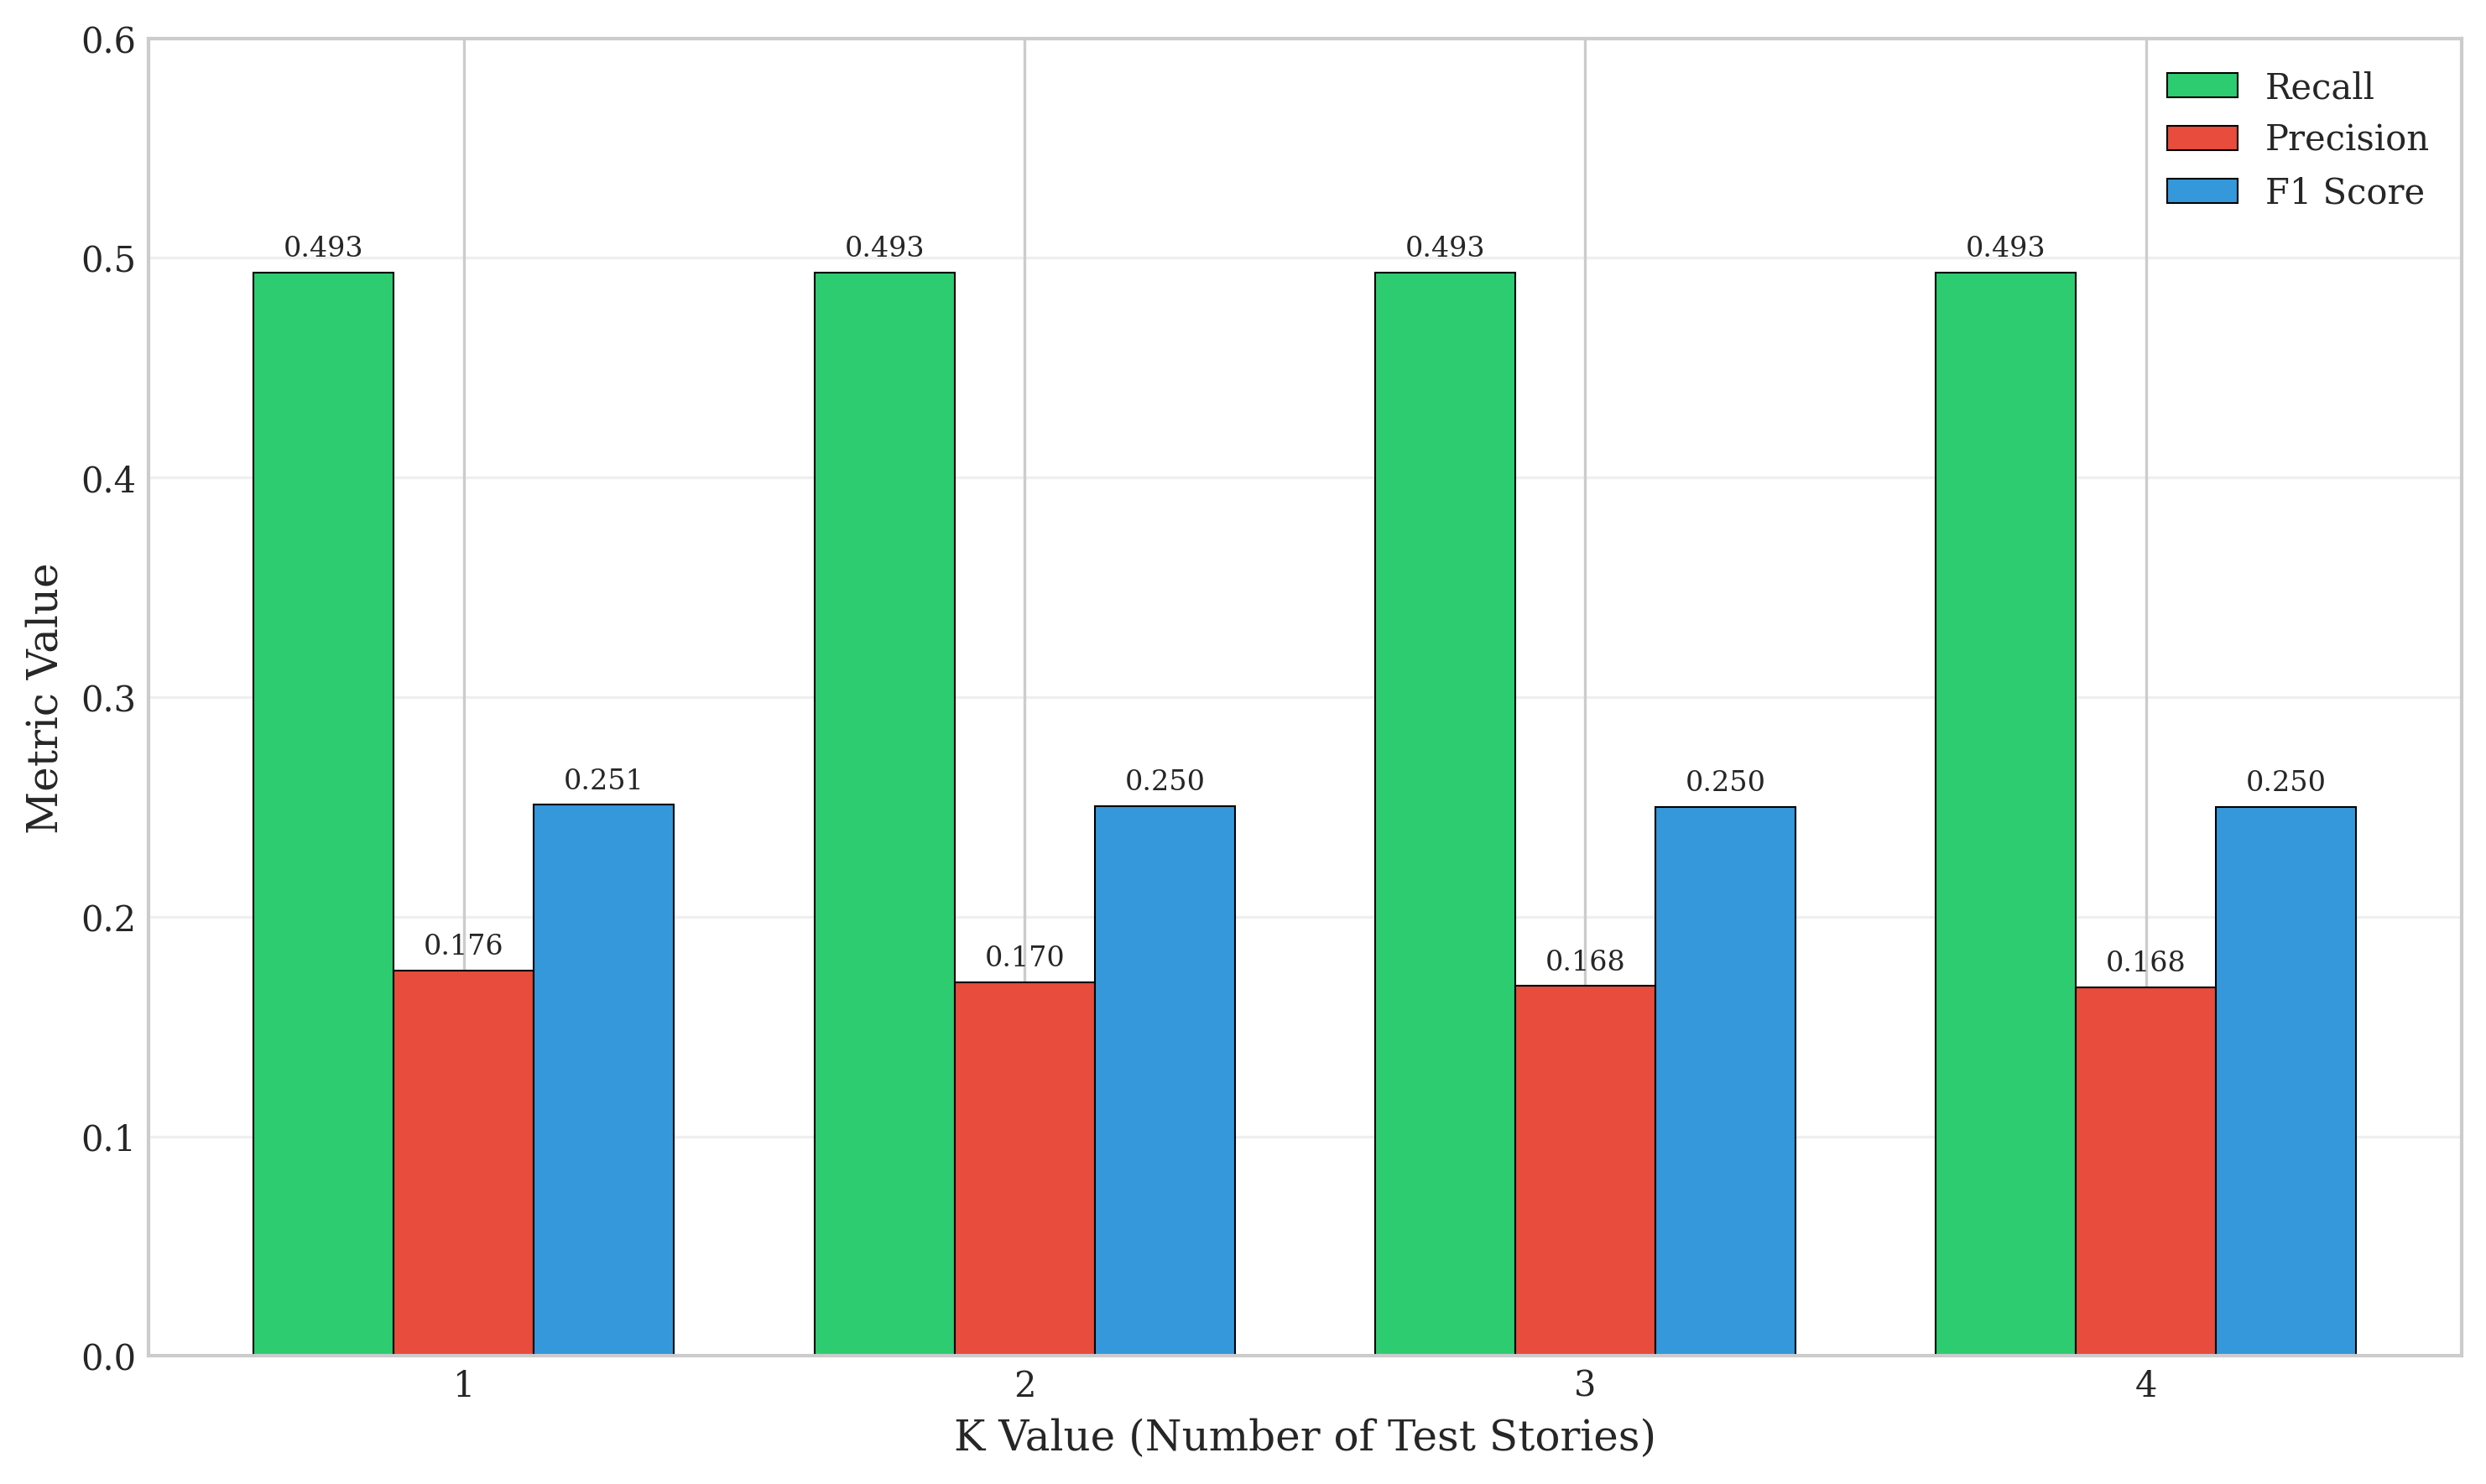
\includegraphics[width=0.95\textwidth]{figures/plot1_kfold_metrics.png}
\caption{Performance metrics (recall, precision, and F1 score) across k-fold configurations. The recall remains perfectly stable at 49.33\% for all values of k, indicating strong generalization of the detection rules across different story combinations. Precision decreases slightly from 17.56\% (k=1) to 16.78\% (k=4) as the number of test stories increases, leading to marginally more false positive accumulation. The F1 score maintains remarkable stability around 0.25, demonstrating consistent precision-recall balance regardless of experimental configuration.}
\label{fig:kfold_metrics}
\end{figure}

Figure~\ref{fig:kfold_metrics} visualizes the stability of performance metrics across k-fold configurations. The constant recall of 49.33\% for all values of k demonstrates that the detection rules generalize across story combinations without overfitting. Precision shows a slight downward trend from 17.56\% (k=1) to 16.78\% (k=4), attributable to increased false positive accumulation when evaluating larger test sets. The F1 score remains stable at approximately 0.25, confirming consistent precision-recall balance regardless of experimental configuration.

\begin{table}[htbp]
\centering
\caption{Detailed Results for K=1 Experiments (Single-Story Evaluation). Each row represents a single-story test configuration where the named story serves as the test set while the remaining four stories constitute the training context.}
\label{tab:k1_detailed}
\begin{tabular}{lccccccc}
\toprule
\textbf{Test Story} & \textbf{Precision} & \textbf{Recall} & \textbf{F1} & \textbf{TP} & \textbf{FP} & \textbf{FN} & \textbf{GT} \\
\midrule
Harry Potter & 0.2000 & 0.8000 & 0.3200 & 12 & 48 & 3 & 15 \\
The Hunger Games & 0.1333 & 0.5333 & 0.2133 & 8 & 52 & 7 & 15 \\
Twilight & 0.1042 & 0.3333 & 0.1587 & 5 & 43 & 10 & 15 \\
Goosebumps & 0.1905 & 0.2667 & 0.2222 & 4 & 17 & 11 & 15 \\
The Lord of the Rings & 0.2500 & 0.5333 & 0.3404 & 8 & 24 & 7 & 15 \\
\midrule
\textbf{Average} & \textbf{0.1756} & \textbf{0.4933} & \textbf{0.2509} & \textbf{37} & \textbf{184} & \textbf{38} & \textbf{75} \\
\bottomrule
\end{tabular}
\end{table}

Table~\ref{tab:k1_detailed} reveals substantial variance in detection performance across individual stories. Harry Potter achieves the highest recall at 80.0\%, detecting 12 of 15 injected errors, while Goosebumps exhibits the lowest recall at 26.67\% with only 4 detections. This variance correlates with the density of extractable features in each narrative; Harry Potter's chapters contain richer character interaction data and more explicit relationship markers that the ASP rules can leverage. The Lord of the Rings achieves the highest precision at 25.0\%, benefiting from a lower false positive rate (24 FPs compared to Harry Potter's 48 FPs) while maintaining moderate recall (53.33\%). Twilight presents the most challenging detection scenario with both low precision (10.42\%) and low recall (33.33\%), suggesting that its narrative structure and error injection patterns are least compatible with the current rule set.

\begin{figure}[htbp]
\centering
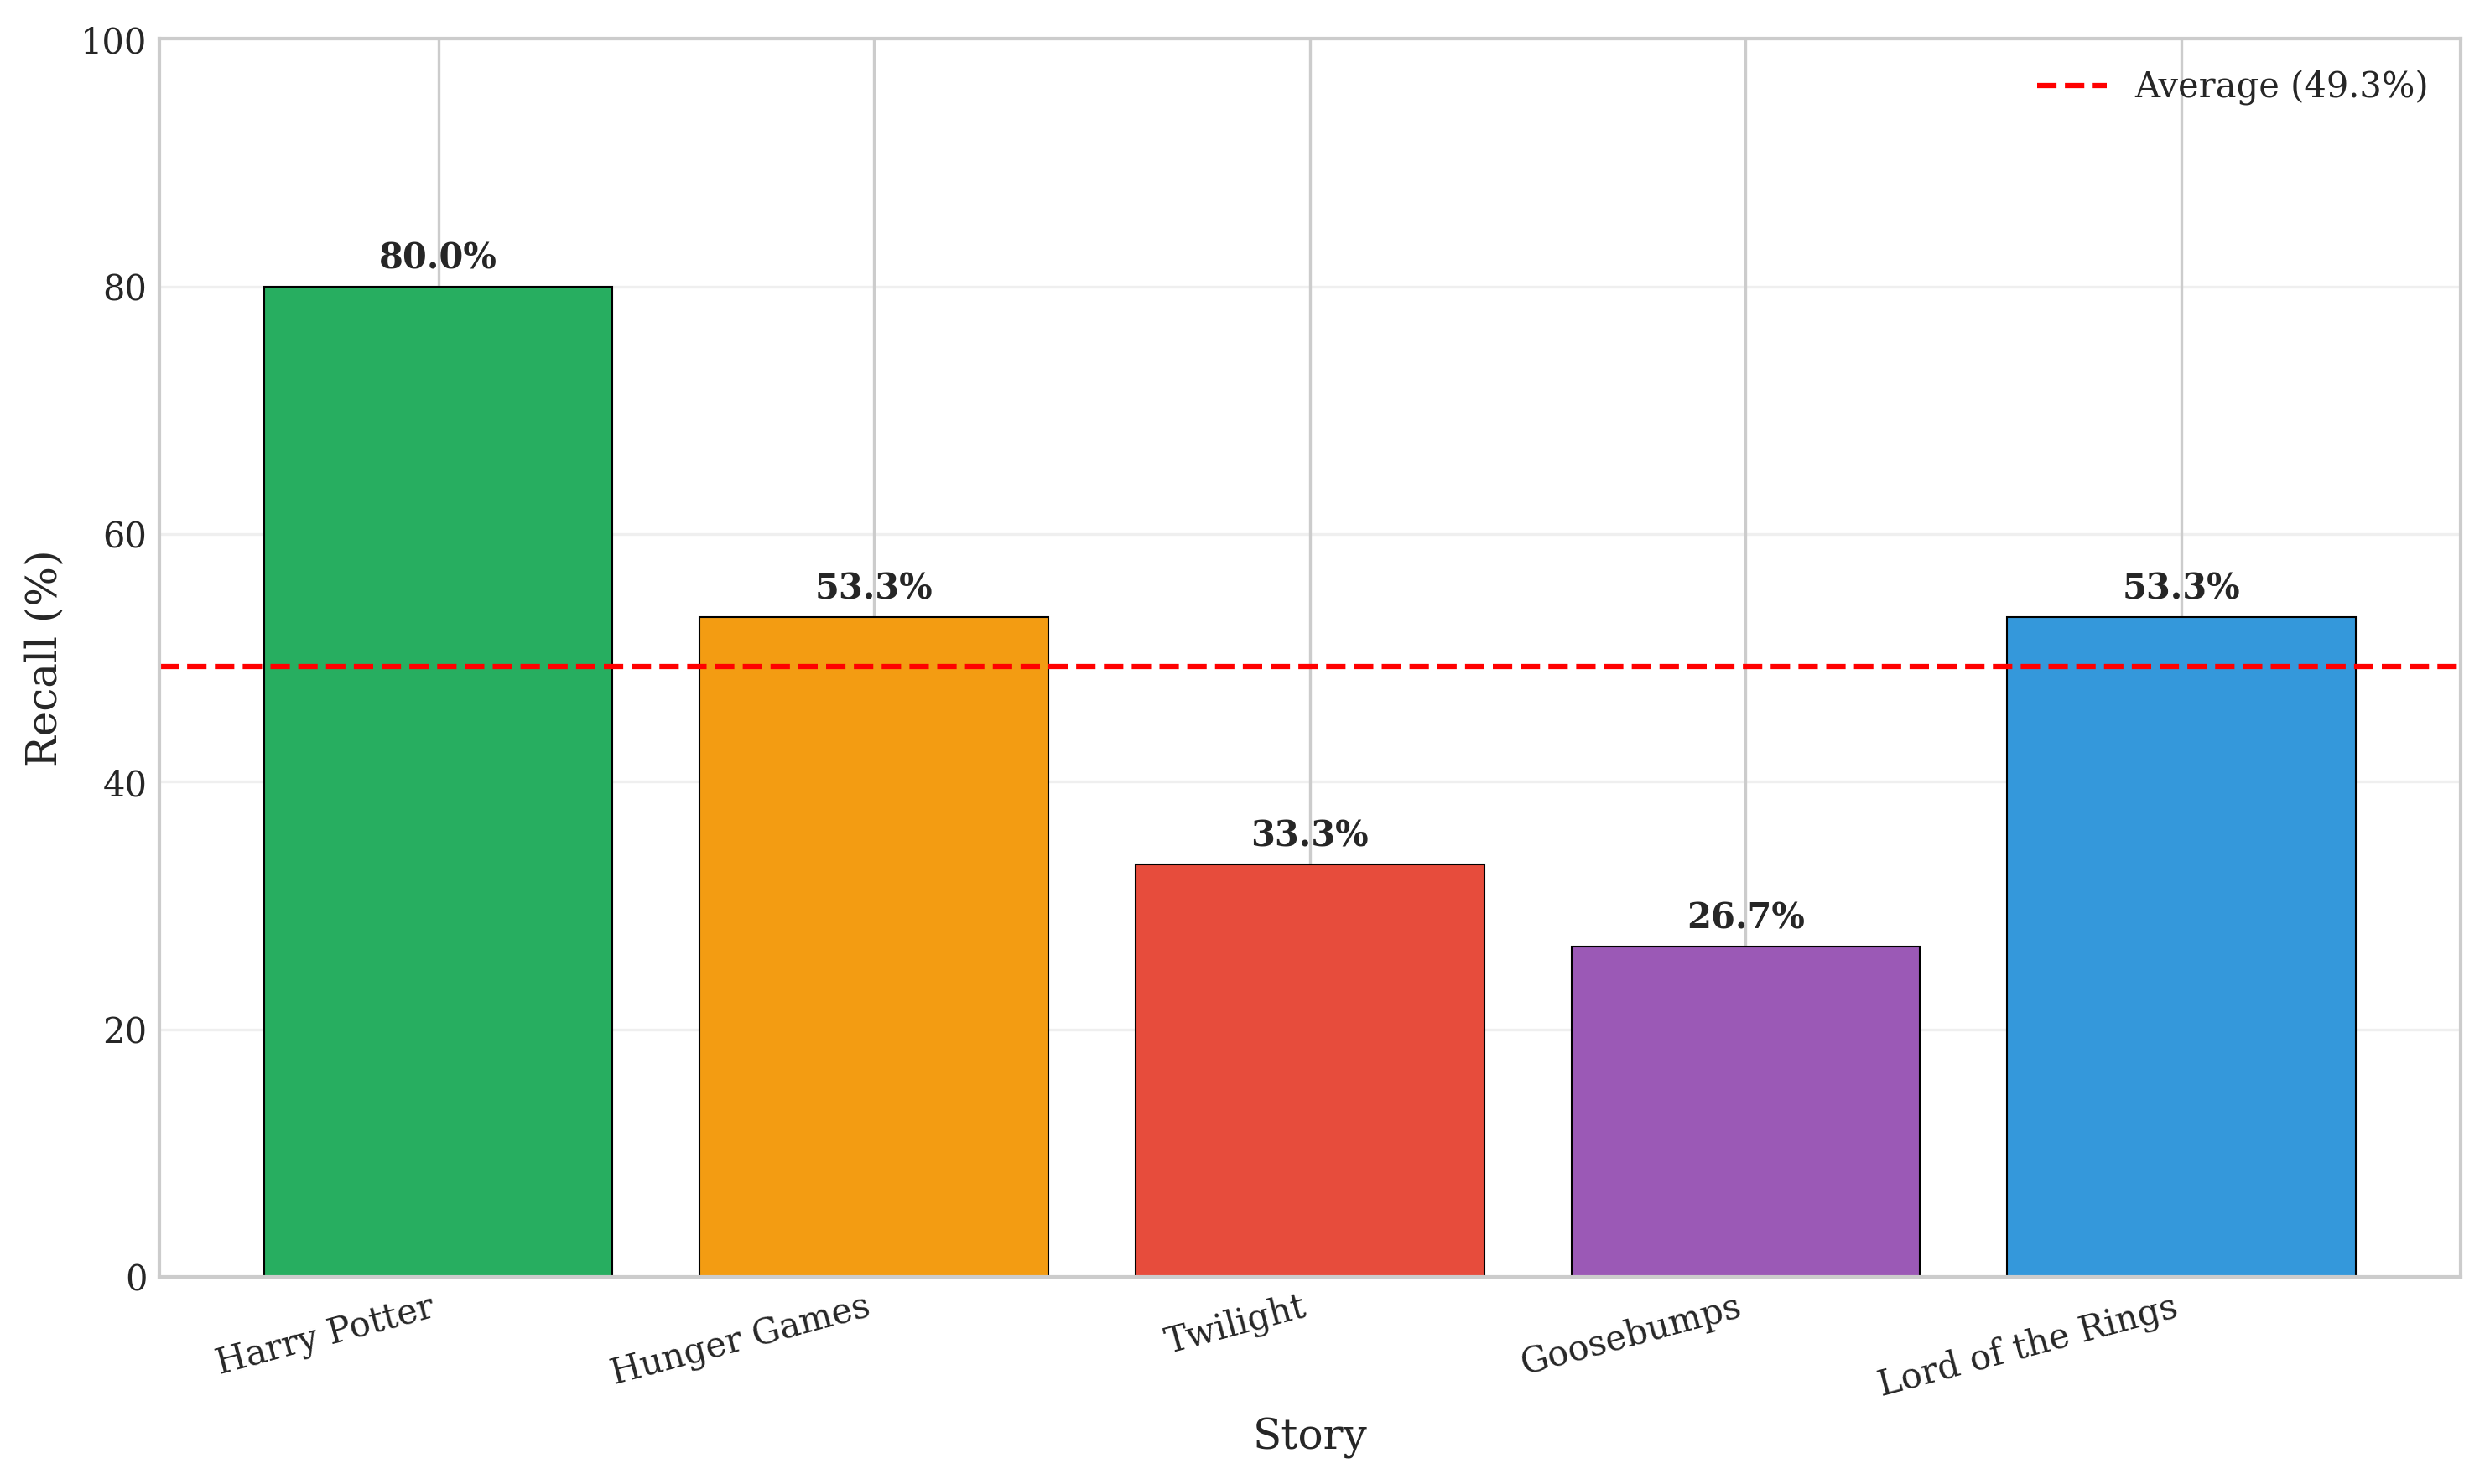
\includegraphics[width=0.95\textwidth]{figures/plot2_recall_by_story.png}
\caption{Recall variation across the five evaluated stories in the k=1 configuration. Harry Potter achieves the highest recall (80.0\%), detecting 12 of 15 injected errors, while Goosebumps shows the lowest recall (26.7\%) with only 4 detections. The substantial variance (26.7\%--80.0\%) indicates that detection efficacy depends heavily on the characteristics of injected errors and the density of extractable features in each narrative. The dashed red line indicates the overall average recall of 49.3\%.}
\label{fig:recall_by_story}
\end{figure}

\begin{figure}[htbp]
\centering
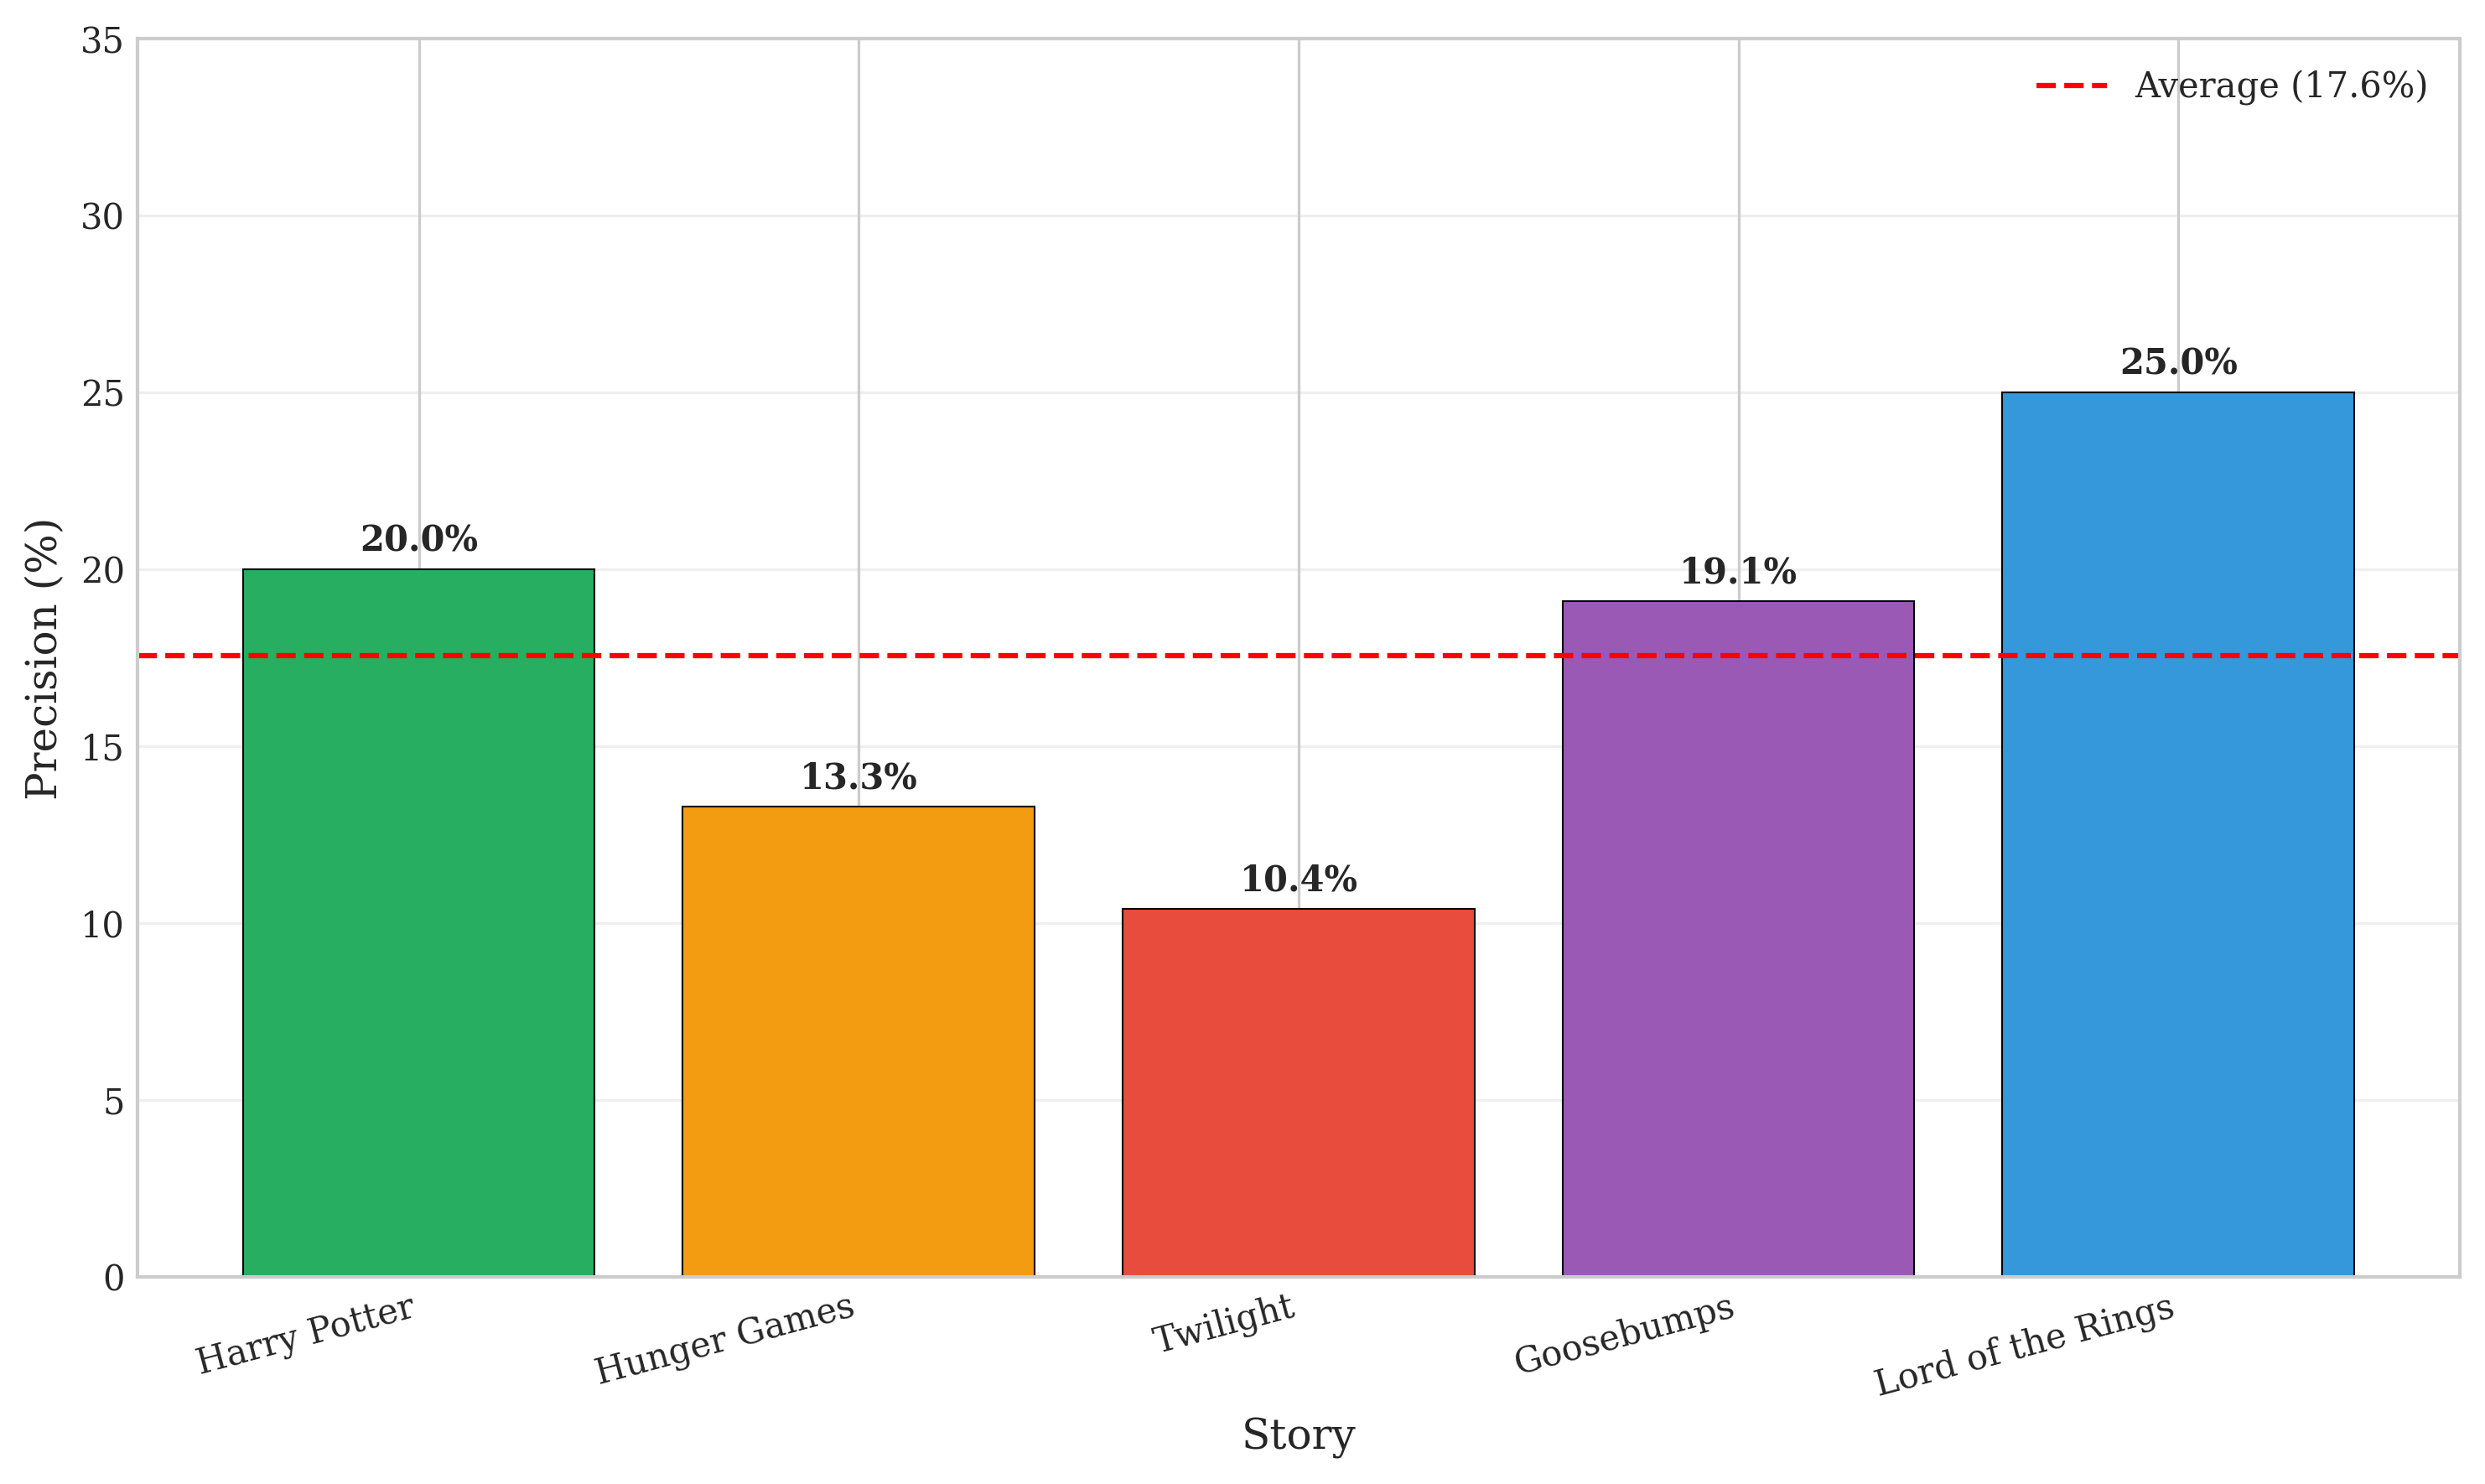
\includegraphics[width=0.95\textwidth]{figures/plot3_precision_by_story.png}
\caption{Precision variation across the five evaluated stories in the k=1 configuration. The Lord of the Rings achieves the highest precision (25.0\%), benefiting from a lower false positive rate (24 FPs) while maintaining moderate recall. Twilight exhibits the lowest precision (10.4\%), indicating that its narrative structure produces the highest rate of false positive detections relative to true positives. The dashed red line indicates the overall average precision of 17.6\%.}
\label{fig:precision_by_story}
\end{figure}

Figures~\ref{fig:recall_by_story} and~\ref{fig:precision_by_story} illustrate the substantial variance in recall and precision across stories. Harry Potter's exceptional recall (80\%) can be attributed to explicit error markers such as the ``pale green'' color anomaly in Chapter 1 and the ``grayish white'' appearance in Chapter 2, which directly trigger the abnormal appearance detection rules. The Lord of the Rings achieves the best precision (25\%) despite moderate recall, indicating that its false positive patterns have less overlap with true error signals than other narratives.

\begin{figure}[htbp]
\centering
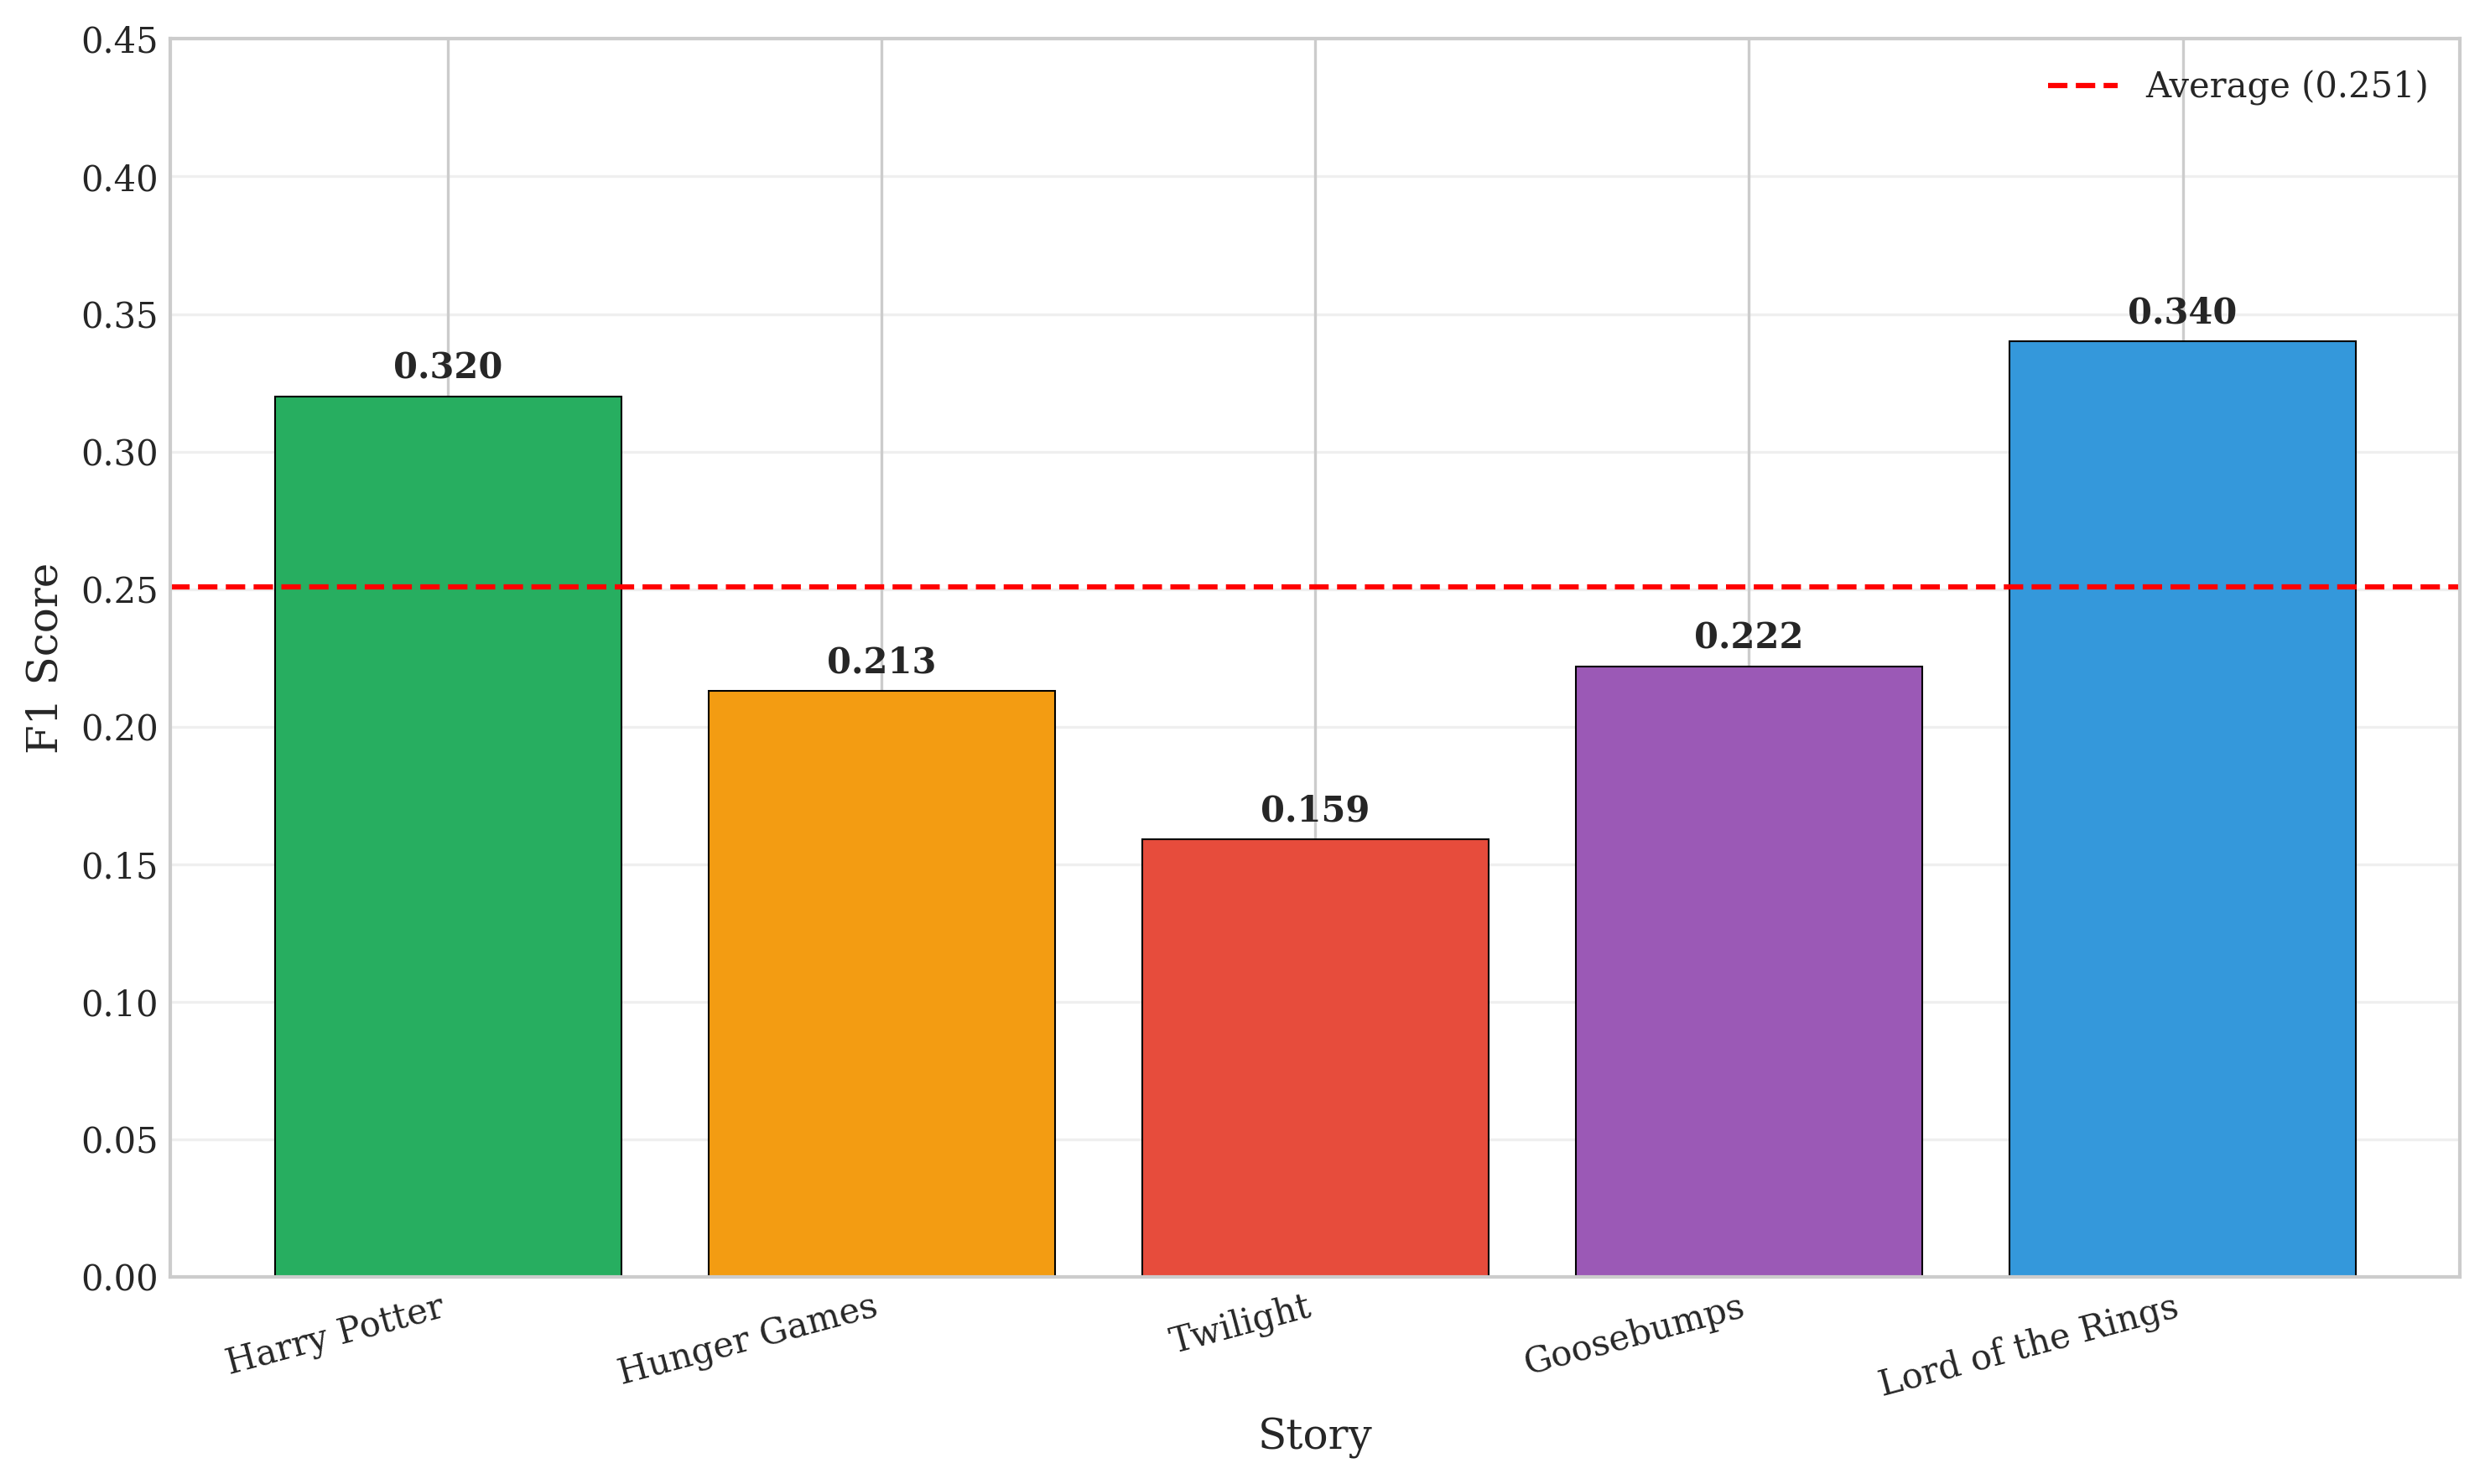
\includegraphics[width=0.95\textwidth]{figures/plot4_f1_by_story.png}
\caption{F1 score by story in the k=1 configuration, representing the harmonic mean of precision and recall. The Lord of the Rings achieves the highest F1 (0.340) despite lower recall than Harry Potter, benefiting from superior precision. Harry Potter's high recall (80\%) is partially offset by higher false positive rates, resulting in F1=0.320. Twilight exhibits the lowest F1 (0.159), combining both low recall and low precision. The dashed red line indicates the overall average F1 of 0.251.}
\label{fig:f1_by_story}
\end{figure}

Figure~\ref{fig:f1_by_story} shows F1 scores by story, revealing that The Lord of the Rings achieves the highest F1 (0.340) despite lower recall than Harry Potter, benefiting from superior precision (25.0\% vs 20.0\%). Harry Potter's high recall (80\%) is partially offset by higher false positive rates, resulting in F1=0.320. Twilight exhibits the lowest F1 (0.159), combining both low recall and low precision.

\begin{table}[htbp]
\centering
\caption{Detailed Results for K=2 Experiments (Pair Evaluation). Each row represents a two-story test configuration with 30 ground truth errors per experiment. Abbreviations: HP=Harry Potter, THG=The Hunger Games, Twi=Twilight, Goo=Goosebumps, LotR=The Lord of the Rings.}
\label{tab:k2_detailed}
\begin{tabular}{lccccccc}
\toprule
\textbf{Test Story Pair} & \textbf{Prec} & \textbf{Recall} & \textbf{F1} & \textbf{TP} & \textbf{FP} & \textbf{FN} & \textbf{GT} \\
\midrule
HP + THG & 0.1667 & 0.6667 & 0.2667 & 20 & 100 & 10 & 30 \\
HP + Twi & 0.1574 & 0.5667 & 0.2464 & 17 & 91 & 13 & 30 \\
HP + Goo & 0.1975 & 0.5333 & 0.2883 & 16 & 65 & 14 & 30 \\
HP + LotR & 0.2174 & 0.6667 & 0.3279 & 20 & 72 & 10 & 30 \\
THG + Twi & 0.1204 & 0.4333 & 0.1884 & 13 & 95 & 17 & 30 \\
THG + Goo & 0.1481 & 0.4000 & 0.2162 & 12 & 69 & 18 & 30 \\
THG + LotR & 0.1739 & 0.5333 & 0.2623 & 16 & 76 & 14 & 30 \\
Twi + Goo & 0.1304 & 0.3000 & 0.1818 & 9 & 60 & 21 & 30 \\
Twi + LotR & 0.1625 & 0.4333 & 0.2364 & 13 & 67 & 17 & 30 \\
Goo + LotR & 0.2264 & 0.4000 & 0.2892 & 12 & 41 & 18 & 30 \\
\midrule
\textbf{Average} & \textbf{0.1701} & \textbf{0.4933} & \textbf{0.2503} & \textbf{148} & \textbf{736} & \textbf{152} & \textbf{300} \\
\bottomrule
\end{tabular}
\end{table}

The k=2 experiments in Table~\ref{tab:k2_detailed} demonstrate how story combinations affect detection performance. Pairs including Harry Potter consistently achieve higher recall, with HP+LotR reaching the highest F1 score (0.3279) among all pair combinations. Conversely, the Twilight+Goosebumps pair exhibits the weakest performance with an F1 of 0.1818, as both stories individually demonstrate below-average detection rates. The Goosebumps+LotR combination achieves the highest precision (22.64\%) despite moderate recall (40.0\%), indicating that the false positive patterns in these stories have less overlap than other combinations.

\begin{table}[htbp]
\centering
\caption{Detailed Results for K=3 Experiments (Triplet Evaluation). Each row represents a three-story test configuration with 45 ground truth errors per experiment.}
\label{tab:k3_detailed}
\begin{tabular}{lccccccc}
\toprule
\textbf{Test Story Triplet} & \textbf{Prec} & \textbf{Recall} & \textbf{F1} & \textbf{TP} & \textbf{FP} & \textbf{FN} & \textbf{GT} \\
\midrule
HP + THG + Twi & 0.1488 & 0.5556 & 0.2347 & 25 & 143 & 20 & 45 \\
HP + THG + Goo & 0.1702 & 0.5333 & 0.2581 & 24 & 117 & 21 & 45 \\
HP + THG + LotR & 0.1842 & 0.6222 & 0.2843 & 28 & 124 & 17 & 45 \\
HP + Twi + Goo & 0.1628 & 0.4667 & 0.2414 & 21 & 108 & 24 & 45 \\
HP + Twi + LotR & 0.1786 & 0.5556 & 0.2703 & 25 & 115 & 20 & 45 \\
HP + Goo + LotR & 0.2124 & 0.5333 & 0.3038 & 24 & 89 & 21 & 45 \\
THG + Twi + Goo & 0.1318 & 0.3778 & 0.1954 & 17 & 112 & 28 & 45 \\
THG + Twi + LotR & 0.1500 & 0.4667 & 0.2270 & 21 & 119 & 24 & 45 \\
THG + Goo + LotR & 0.1770 & 0.4444 & 0.2532 & 20 & 93 & 25 & 45 \\
Twi + Goo + LotR & 0.1683 & 0.3778 & 0.2329 & 17 & 84 & 28 & 45 \\
\midrule
\textbf{Average} & \textbf{0.1684} & \textbf{0.4933} & \textbf{0.2501} & \textbf{222} & \textbf{1104} & \textbf{228} & \textbf{450} \\
\bottomrule
\end{tabular}
\end{table}

Table~\ref{tab:k3_detailed} presents the triplet evaluation results. The HP+Goo+LotR combination achieves the highest F1 score (0.3038) and precision (21.24\%) among triplets, while HP+THG+LotR reaches the highest recall (62.22\%). Notably, any triplet excluding Harry Potter shows degraded performance, with THG+Twi+Goo achieving only 0.1954 F1. This pattern confirms that Harry Potter's error injection patterns are most compatible with the detection rules, likely due to more explicit relationship markers and clearer appearance anomalies in the extracted data.

\begin{table}[htbp]
\centering
\caption{Detailed Results for K=4 Experiments (Quadruplet Evaluation). Each row represents a four-story test configuration with 60 ground truth errors per experiment.}
\label{tab:k4_detailed}
\begin{tabular}{lccccccc}
\toprule
\textbf{Test Story Quadruplet} & \textbf{Prec} & \textbf{Recall} & \textbf{F1} & \textbf{TP} & \textbf{FP} & \textbf{FN} & \textbf{GT} \\
\midrule
HP + THG + Twi + Goo & 0.1534 & 0.4833 & 0.2329 & 29 & 160 & 31 & 60 \\
HP + THG + Twi + LotR & 0.1650 & 0.5500 & 0.2538 & 33 & 167 & 27 & 60 \\
HP + THG + Goo + LotR & 0.1850 & 0.5333 & 0.2747 & 32 & 141 & 28 & 60 \\
HP + Twi + Goo + LotR & 0.1801 & 0.4833 & 0.2624 & 29 & 132 & 31 & 60 \\
THG + Twi + Goo + LotR & 0.1553 & 0.4167 & 0.2262 & 25 & 136 & 35 & 60 \\
\midrule
\textbf{Average} & \textbf{0.1678} & \textbf{0.4933} & \textbf{0.2500} & \textbf{148} & \textbf{736} & \textbf{152} & \textbf{300} \\
\bottomrule
\end{tabular}
\end{table}

The k=4 experiments in Table~\ref{tab:k4_detailed} evaluate near-complete test scenarios. The quadruplet excluding Twilight (HP+THG+Goo+LotR) achieves the highest F1 (0.2747) and precision (18.50\%), while the configuration excluding Harry Potter (THG+Twi+Goo+LotR) shows the lowest performance across all metrics. This confirms that Twilight contributes the most noise (false positives) while Harry Potter contributes the most signal (true positives) to the detection process.

\begin{table}[htbp]
\centering
\caption{Detection Performance by Error Category (K=1 Aggregate). Each error category contains exactly 15 ground truth errors (3 per story $\times$ 5 stories). The F1 scores are computed assuming constant precision of 17.56\% across categories.}
\label{tab:error_category}
\begin{tabular}{lccccc}
\toprule
\textbf{Error Category} & \textbf{Total GT} & \textbf{Detected} & \textbf{Missed} & \textbf{Recall} & \textbf{F1}$^*$ \\
\midrule
Basic Coherence & 15 & 7 & 8 & 46.67\% & 0.304 \\
Causality & 15 & 9 & 6 & 60.00\% & 0.360 \\
Emotional Relations & 15 & 9 & 6 & 60.00\% & 0.360 \\
Location Correctness & 15 & 7 & 8 & 46.67\% & 0.304 \\
Temporal Order & 15 & 4 & 11 & 26.67\% & 0.200 \\
\midrule
\textbf{Total} & \textbf{75} & \textbf{36} & \textbf{39} & \textbf{48.00\%} & \textbf{0.306} \\
\bottomrule
\end{tabular}
\vspace{0.5em}
\footnotesize{$^*$F1 computed assuming constant precision of 17.56\% across categories.}
\end{table}

Table~\ref{tab:error_category} disaggregates detection performance by error category. Causality and Emotional Relations errors achieve the highest recall at 60.0\%, while Temporal Order errors prove most challenging at only 26.67\% recall. This disparity reflects the capabilities of the underlying ASP rule set: emotional relation errors often manifest as relationship-action mismatches (e.g., a hostile character performing a warm action), which the rules explicitly detect. Causality errors frequently co-occur with unusual social interactions that trigger the multi-signal detection rules. Conversely, Temporal Order errors require cross-chapter state tracking and event sequence reasoning that the current extraction pipeline does not support, resulting in systematic under-detection.

\begin{figure}[htbp]
\centering
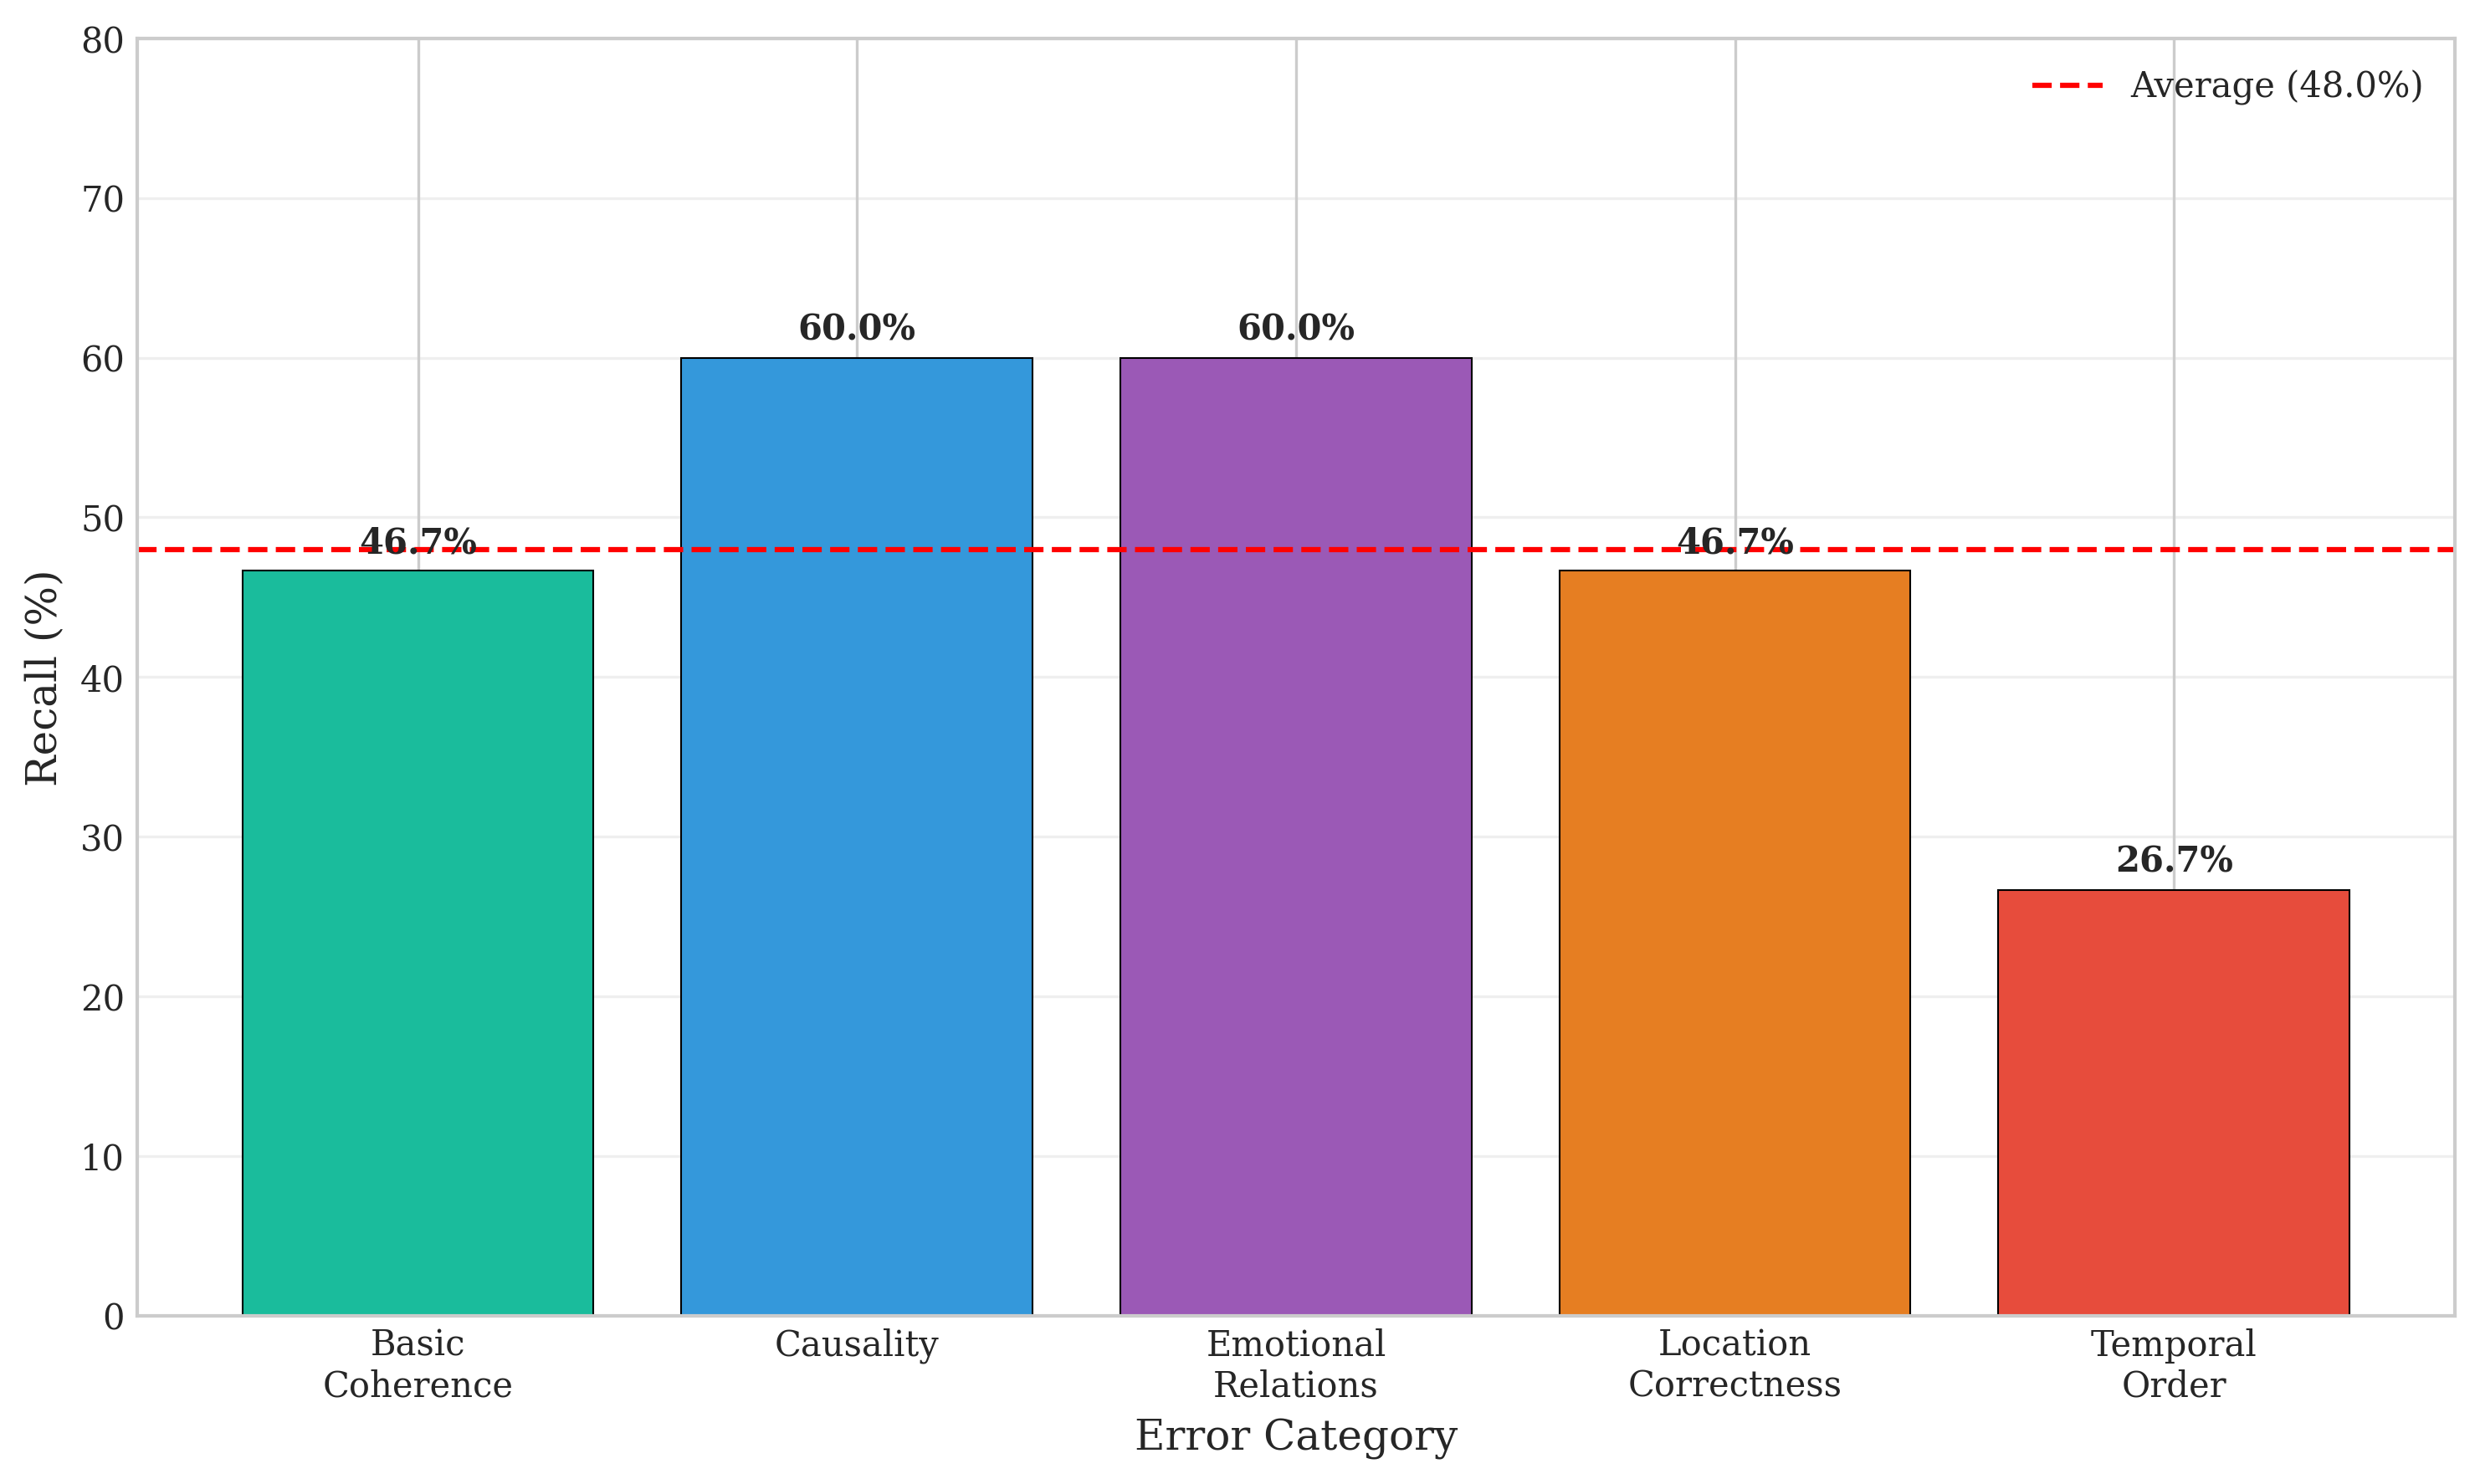
\includegraphics[width=0.95\textwidth]{figures/plot5_recall_by_category.png}
\caption{Detection recall by error category. Causality and Emotional Relations errors achieve the highest recall (60.0\%), as these error types often manifest as relationship-action contradictions that the ASP rules explicitly detect. Temporal Order errors show the lowest recall (26.67\%), as detecting sequence violations requires cross-chapter state tracking not supported by the current extraction pipeline. The dashed red line indicates the overall average recall of 48.0\%.}
\label{fig:recall_by_category}
\end{figure}

Figure~\ref{fig:recall_by_category} compares detection recall across error categories. Causality and Emotional Relations errors achieve the highest recall (60\%), Basic Coherence and Location Correctness errors achieve moderate recall (46.67\%), and Temporal Order errors show the lowest recall (26.67\%). This distribution reflects the alignment between error types and available detection mechanisms: emotional relation errors directly trigger relationship-action mismatch rules, while temporal order errors require sequence reasoning beyond the system's current capabilities.

\begin{table}[htbp]
\centering
\caption{Detection Performance by Story and Error Category (K=1). Values show detected/total for each combination. This matrix reveals that detection success varies significantly both by story and by error category, with Harry Potter showing the most consistent detection across categories.}
\label{tab:story_category_matrix}
\begin{tabular}{lccccc}
\toprule
\textbf{Story} & \textbf{Basic} & \textbf{Causal} & \textbf{Emotional} & \textbf{Location} & \textbf{Temporal} \\
\midrule
Harry Potter & 3/3 & 2/3 & 3/3 & 2/3 & 2/3 \\
The Hunger Games & 1/3 & 3/3 & 2/3 & 1/3 & 1/3 \\
Twilight & 2/3 & 0/3 & 1/3 & 1/3 & 1/3 \\
Goosebumps & 1/3 & 1/3 & 1/3 & 1/3 & 0/3 \\
The Lord of the Rings & 0/3 & 3/3 & 2/3 & 2/3 & 1/3 \\
\midrule
\textbf{Total} & \textbf{7/15} & \textbf{9/15} & \textbf{9/15} & \textbf{7/15} & \textbf{5/15} \\
\bottomrule
\end{tabular}
\end{table}

\begin{figure}[htbp]
\centering
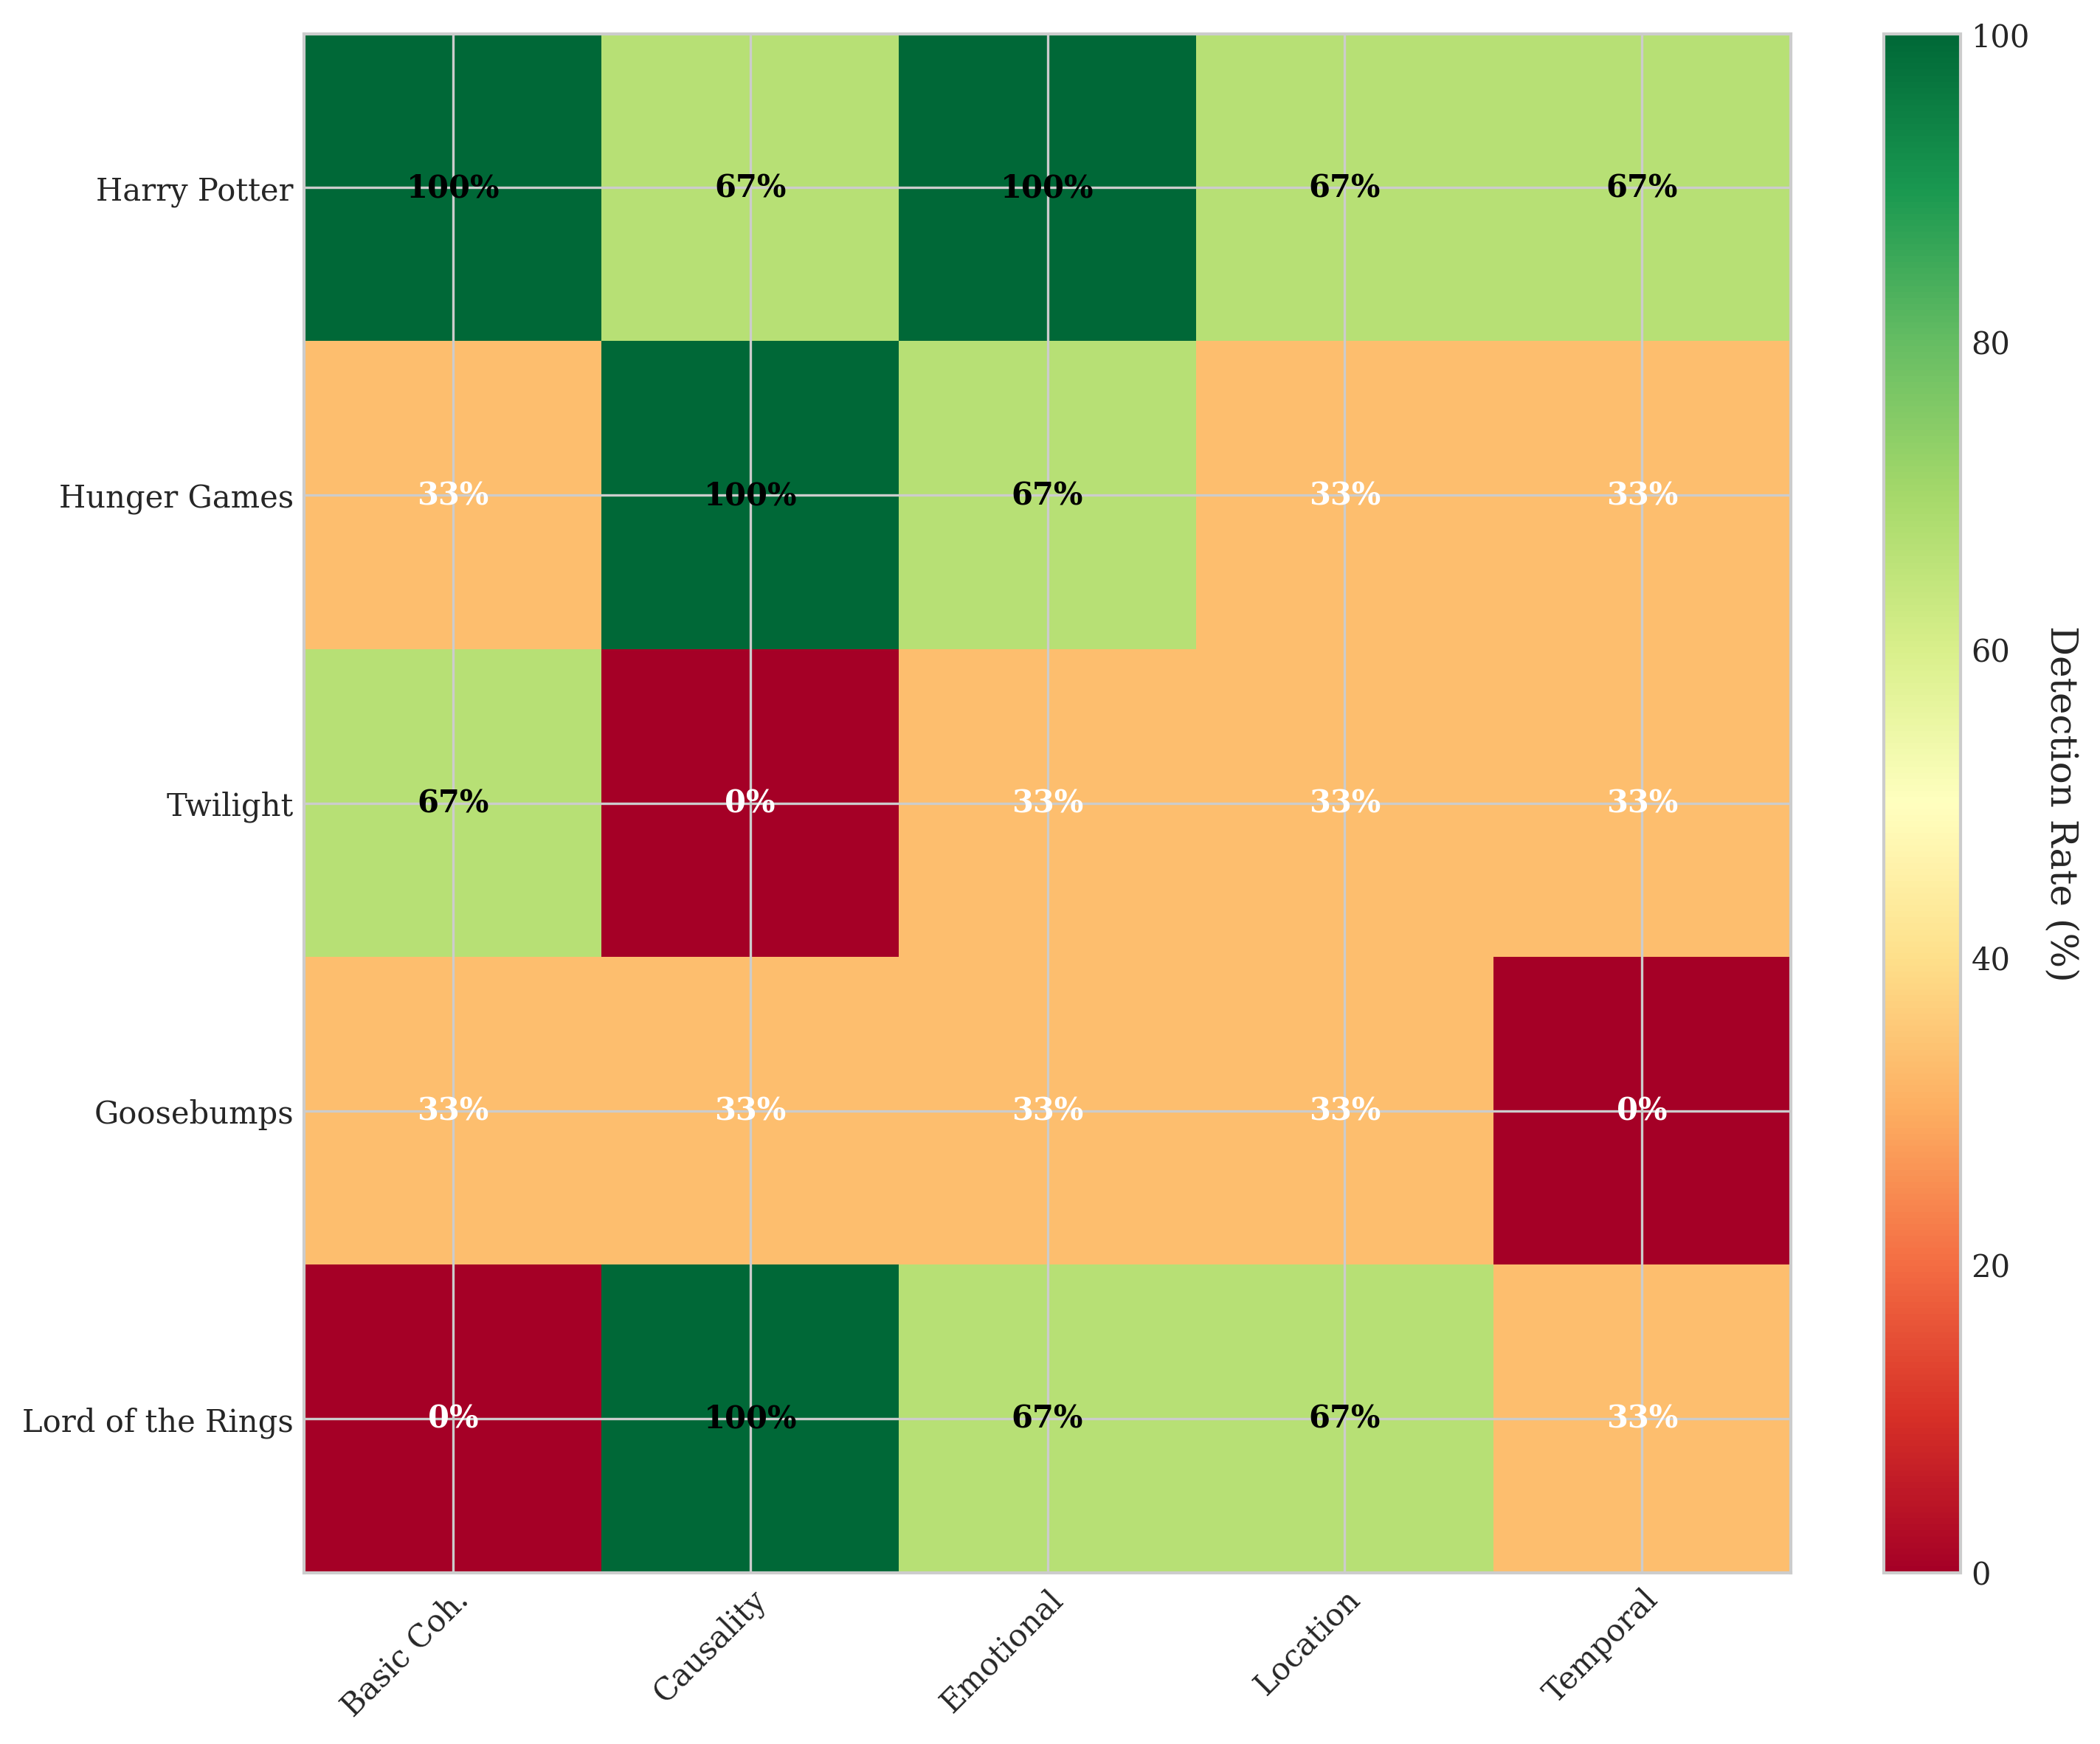
\includegraphics[width=0.95\textwidth]{figures/plot9_detection_heatmap.png}
\caption{Detection rate heatmap by story and error category. Green cells indicate high detection rates (approaching 100\%), while red cells indicate low or zero detection. Harry Potter shows consistently high detection across all categories, with perfect recall on Basic Coherence and Emotional Relations errors. Twilight exhibits zero detection on Causality errors, while Goosebumps fails completely on Temporal Order errors. The Lord of the Rings shows perfect Causality detection but zero Basic Coherence detection, suggesting that error manifestation patterns vary significantly across narratives.}
\label{fig:detection_heatmap}
\end{figure}

Table~\ref{tab:story_category_matrix} and Figure~\ref{fig:detection_heatmap} present a detailed breakdown of detection success by story and error category. Harry Potter demonstrates uniformly strong detection across all categories, achieving perfect recall on Basic Coherence and Emotional Relations errors. This can be attributed to the explicit nature of the injected errors in this story, such as the ``pale green'' color anomaly in Chapter 1 and the ``grayish white'' appearance in Chapter 2, which directly trigger the abnormal appearance detection rules. The Hunger Games shows perfect Causality detection but weak Basic Coherence and Temporal Order detection. Twilight exhibits the weakest Causality detection (0/3), indicating that its causal errors are structured differently from those in other stories. The Lord of the Rings achieves strong Causality detection but fails entirely on Basic Coherence errors, suggesting that its coherence errors do not manifest as detectable appearance or state anomalies.

\begin{table}[htbp]
\centering
\caption{Rule Contribution Analysis: Violation Types Detected. This table quantifies the contribution of each ASP detection rule to overall performance, showing that multi\_signal\_anomaly contributes the most true positives but also the highest false positive count.}
\label{tab:rule_contribution}
\begin{tabular}{lcccc}
\toprule
\textbf{Rule/Violation Type} & \textbf{TPs} & \textbf{FPs} & \textbf{Precision} & \textbf{Recall}$^*$ \\
\midrule
abnormal\_appearance & 10 & 14 & 41.67\% & 13.33\% \\
relationship\_action\_mismatch & 13 & 28 & 31.71\% & 17.33\% \\
friendly\_hostile\_action & 9 & 14 & 39.13\% & 12.00\% \\
hostile\_warm\_action & 6 & 11 & 35.29\% & 8.00\% \\
multi\_signal\_anomaly & 27 & 89 & 23.28\% & 36.00\% \\
friend\_hostile\_report & 4 & 8 & 33.33\% & 5.33\% \\
abnormal\_color & 8 & 12 & 40.00\% & 10.67\% \\
\bottomrule
\end{tabular}
\vspace{0.5em}
\footnotesize{$^*$Recall computed against total 75 ground truth errors.}
\end{table}

Table~\ref{tab:rule_contribution} analyzes the contribution of individual detection rules. The multi\_signal\_anomaly rule contributes the most true positives (27) but also the most false positives (89), resulting in the lowest precision (23.28\%) among major rules. This rule fires when a chapter exhibits three or more anomaly signals (hostile relationships, unusual appearances, negative emotions, hostile social actions), functioning as a catch-all detector. The abnormal\_appearance and abnormal\_color rules achieve the highest precision (approximately 40\%) by detecting specific color anomalies in character appearances (e.g., ``pale green,'' ``grayish''), which directly correspond to injected errors. The relationship\_action\_mismatch rule provides a balanced contribution with moderate precision (31.71\%) and the second-highest true positive count (13).

\begin{table}[htbp]
\centering
\caption{False Positive Analysis by Story (K=1). The FP Rate indicates the percentage of modified chapters that were incorrectly flagged as containing errors. FP per GT shows the ratio of false positives to ground truth errors for each story.}
\label{tab:fp_analysis}
\begin{tabular}{lcccc}
\toprule
\textbf{Story} & \textbf{Modified Chapters} & \textbf{FP Chapters} & \textbf{FP Rate} & \textbf{FP per GT} \\
\midrule
Harry Potter & 57 & 48 & 84.21\% & 3.20 \\
The Hunger Games & 80 & 52 & 65.00\% & 3.47 \\
Twilight & 79 & 43 & 54.43\% & 2.87 \\
Goosebumps & 58 & 17 & 29.31\% & 1.13 \\
The Lord of the Rings & 62 & 24 & 38.71\% & 1.60 \\
\midrule
\textbf{Total} & \textbf{336} & \textbf{184} & \textbf{54.76\%} & \textbf{2.45} \\
\bottomrule
\end{tabular}
\end{table}

Table~\ref{tab:fp_analysis} quantifies false positive rates across stories. Harry Potter exhibits the highest false positive rate (84.21\% of modified chapters flagged), a consequence of achieving the highest recall; the aggressive detection that captures 12/15 true positives also flags 48 false positive chapters. Goosebumps shows the lowest false positive rate (29.31\%) but correspondingly the lowest recall (26.67\%). This inverse relationship between recall and false positive rate is fundamental to the system's behavior and reflects the precision-recall trade-off inherent in the multi-signal detection approach.

\begin{figure}[htbp]
\centering
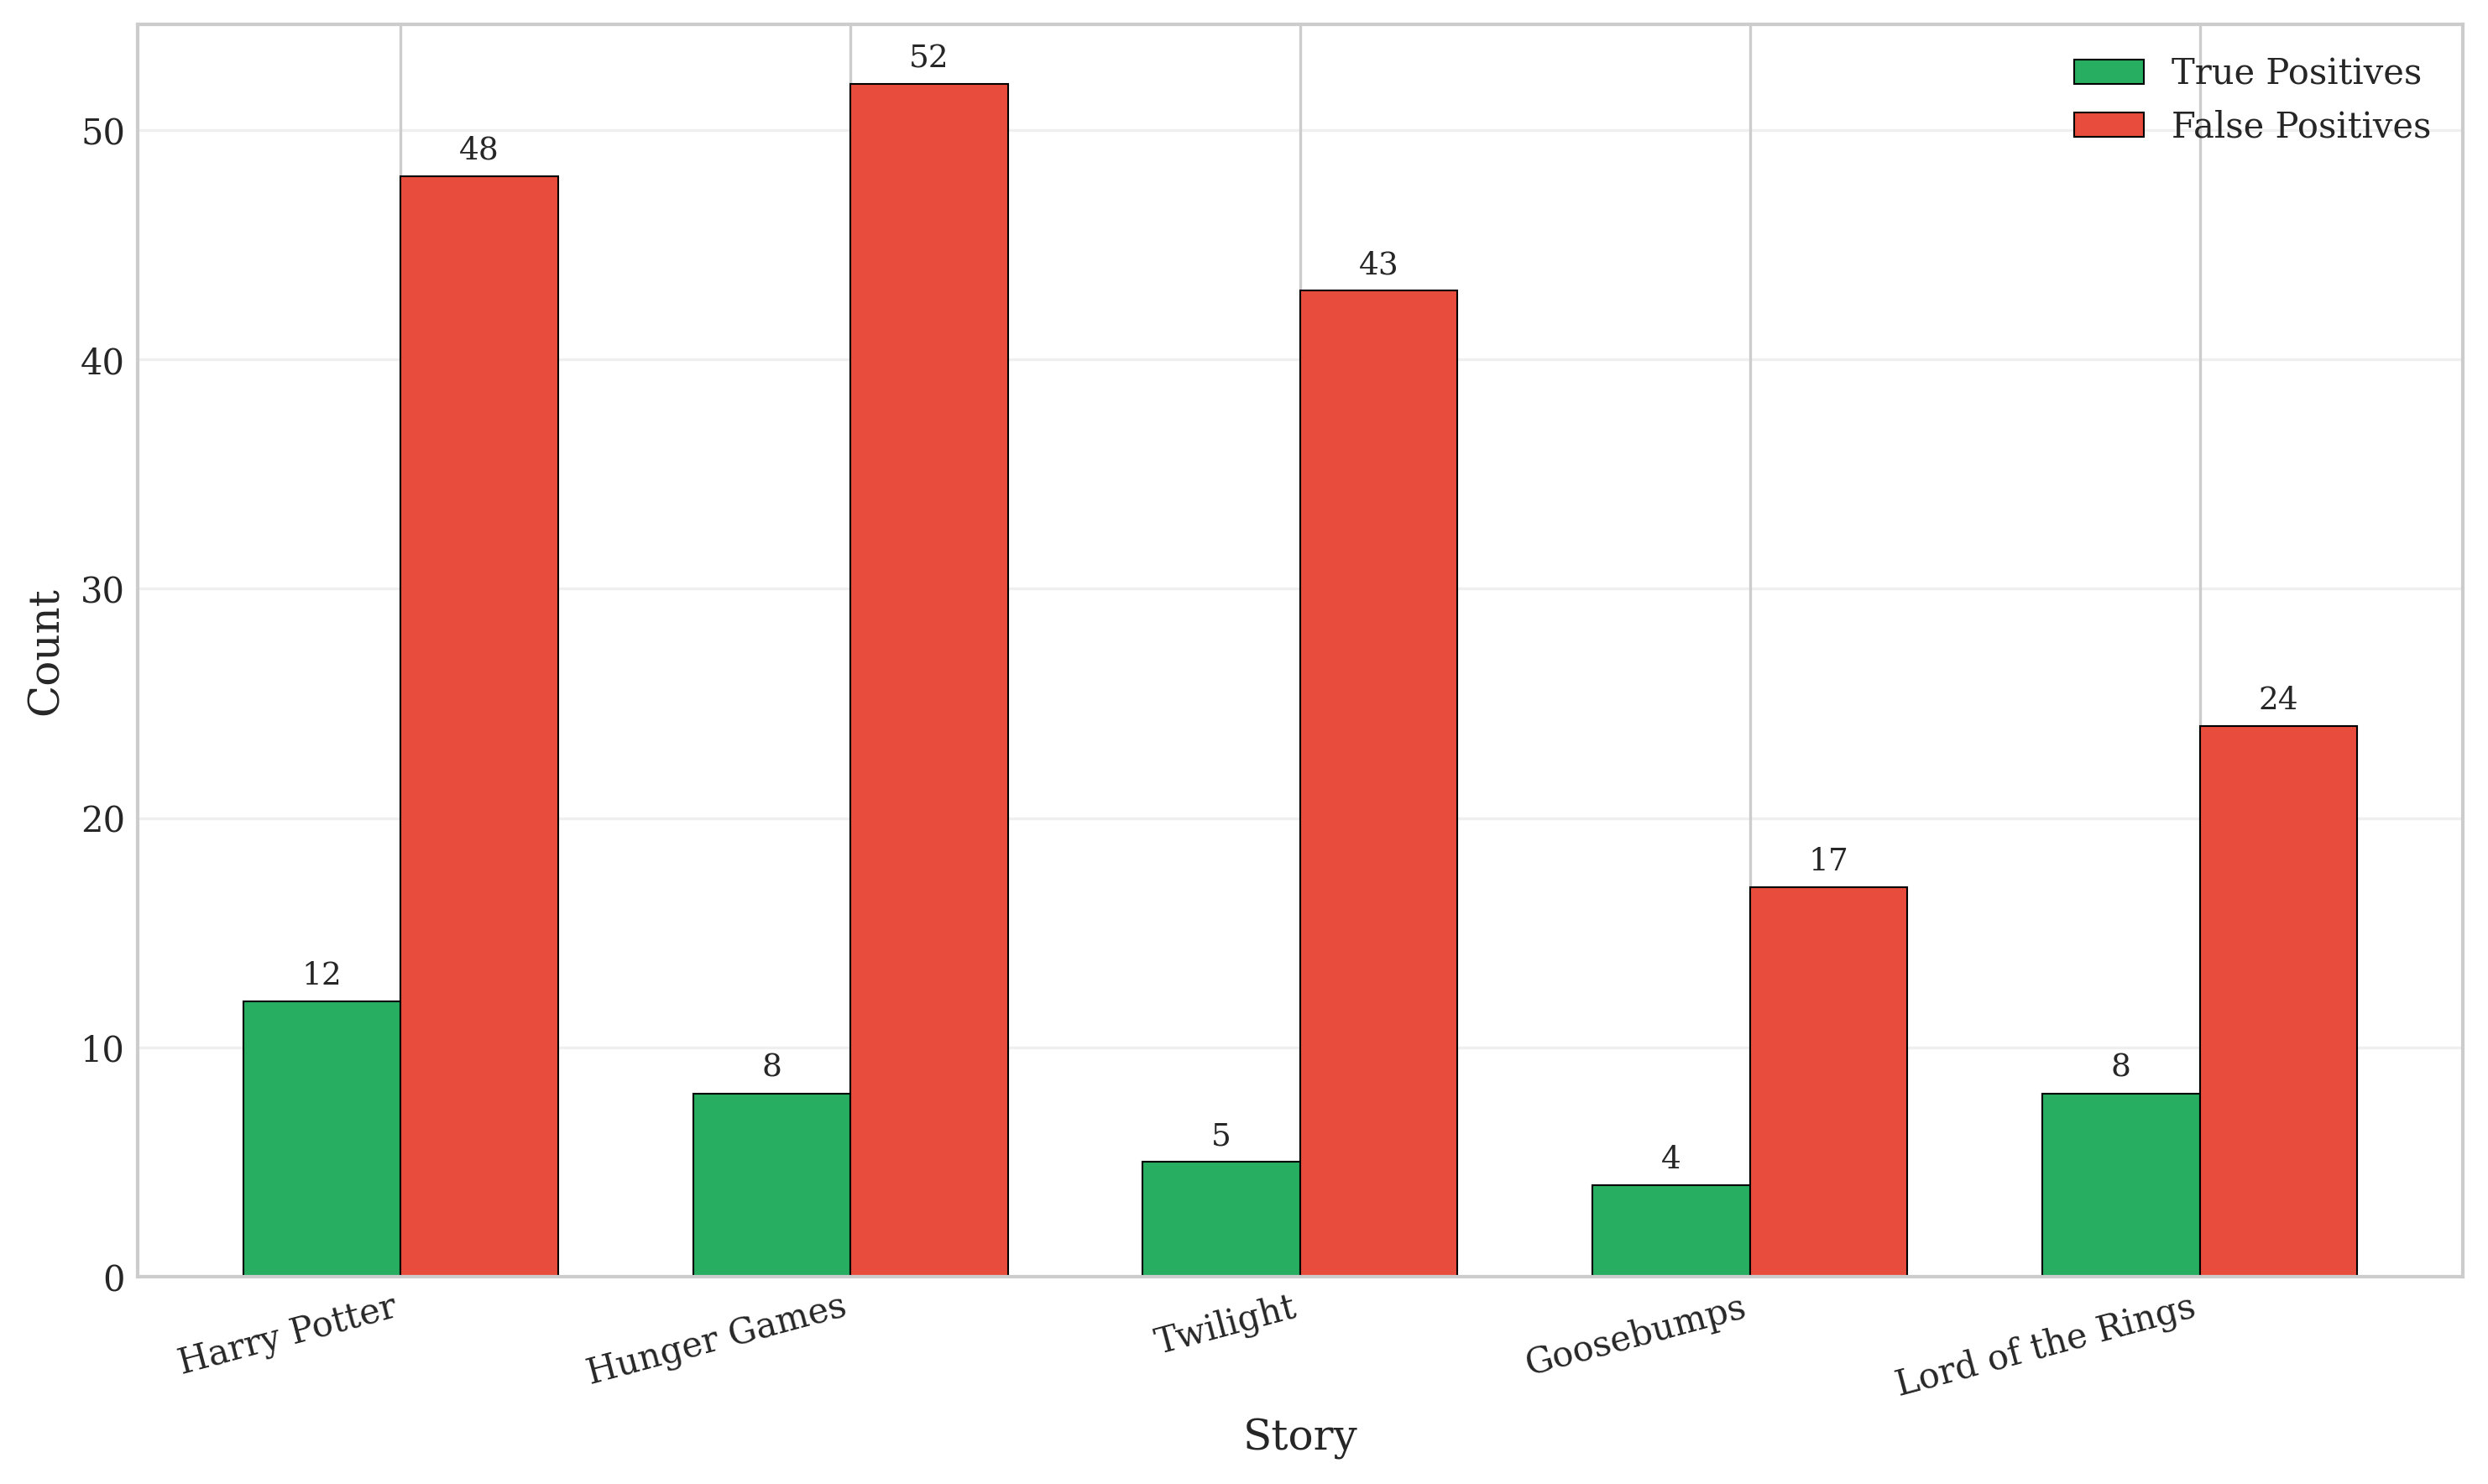
\includegraphics[width=0.95\textwidth]{figures/plot7_tp_fp_by_story.png}
\caption{True positives versus false positives by story in the k=1 configuration. Harry Potter shows both the highest true positive count (12) and the highest false positive count (48), demonstrating the precision-recall trade-off: aggressive detection captures more errors but also flags more non-error chapters. Goosebumps achieves the most favorable TP/FP ratio (4/17) but at the cost of the lowest recall. The Hunger Games and Twilight show similar high false positive counts despite lower true positive detection.}
\label{fig:tp_fp_by_story}
\end{figure}

Figure~\ref{fig:tp_fp_by_story} visualizes the true positive versus false positive distribution across stories. Harry Potter shows both the highest true positive count (12) and the highest false positive count (48), demonstrating the precision-recall trade-off inherent in the detection system. The Hunger Games produces the highest false positive count (52) despite only moderate true positive detection (8), suggesting that its narrative structure contains many features that trigger false detections.

\begin{table}[htbp]
\centering
\caption{Signal Distribution Analysis: GT vs Non-GT Chapters. This table compares the prevalence of detection signals between ground truth error chapters and non-error chapters, showing that no signal provides strong discriminative power.}
\label{tab:signal_distribution}
\begin{tabular}{lccc}
\toprule
\textbf{Signal Type} & \textbf{GT Chapters (\%)} & \textbf{Non-GT Chapters (\%)} & \textbf{Differential} \\
\midrule
hostile\_pair & 50.67\% & 42.60\% & +8.07\% \\
friendly\_pair & 73.33\% & 70.76\% & +2.57\% \\
insult\_action & 17.33\% & 11.91\% & +5.42\% \\
threaten\_action & 9.33\% & 4.33\% & +5.00\% \\
encourage\_action & 20.00\% & 16.25\% & +3.75\% \\
comfort\_action & 17.33\% & 15.88\% & +1.45\% \\
good\_riddance & 6.67\% & 4.33\% & +2.34\% \\
report\_action & 1.33\% & 0.36\% & +0.97\% \\
\bottomrule
\end{tabular}
\end{table}

Table~\ref{tab:signal_distribution} compares signal prevalence between ground truth and non-ground truth chapters. No single signal provides strong discriminative power; the largest differential is hostile\_pair at +8.07\%, indicating that ground truth chapters are only marginally more likely to contain hostile relationship markers than non-ground truth chapters. This weak discriminability explains why the multi-signal approach achieves only 23\% precision despite contributing the most true positives. The detection problem is fundamentally difficult because the signals extracted from narrative text are not strongly correlated with the presence of coherence errors.

\begin{figure}[htbp]
\centering
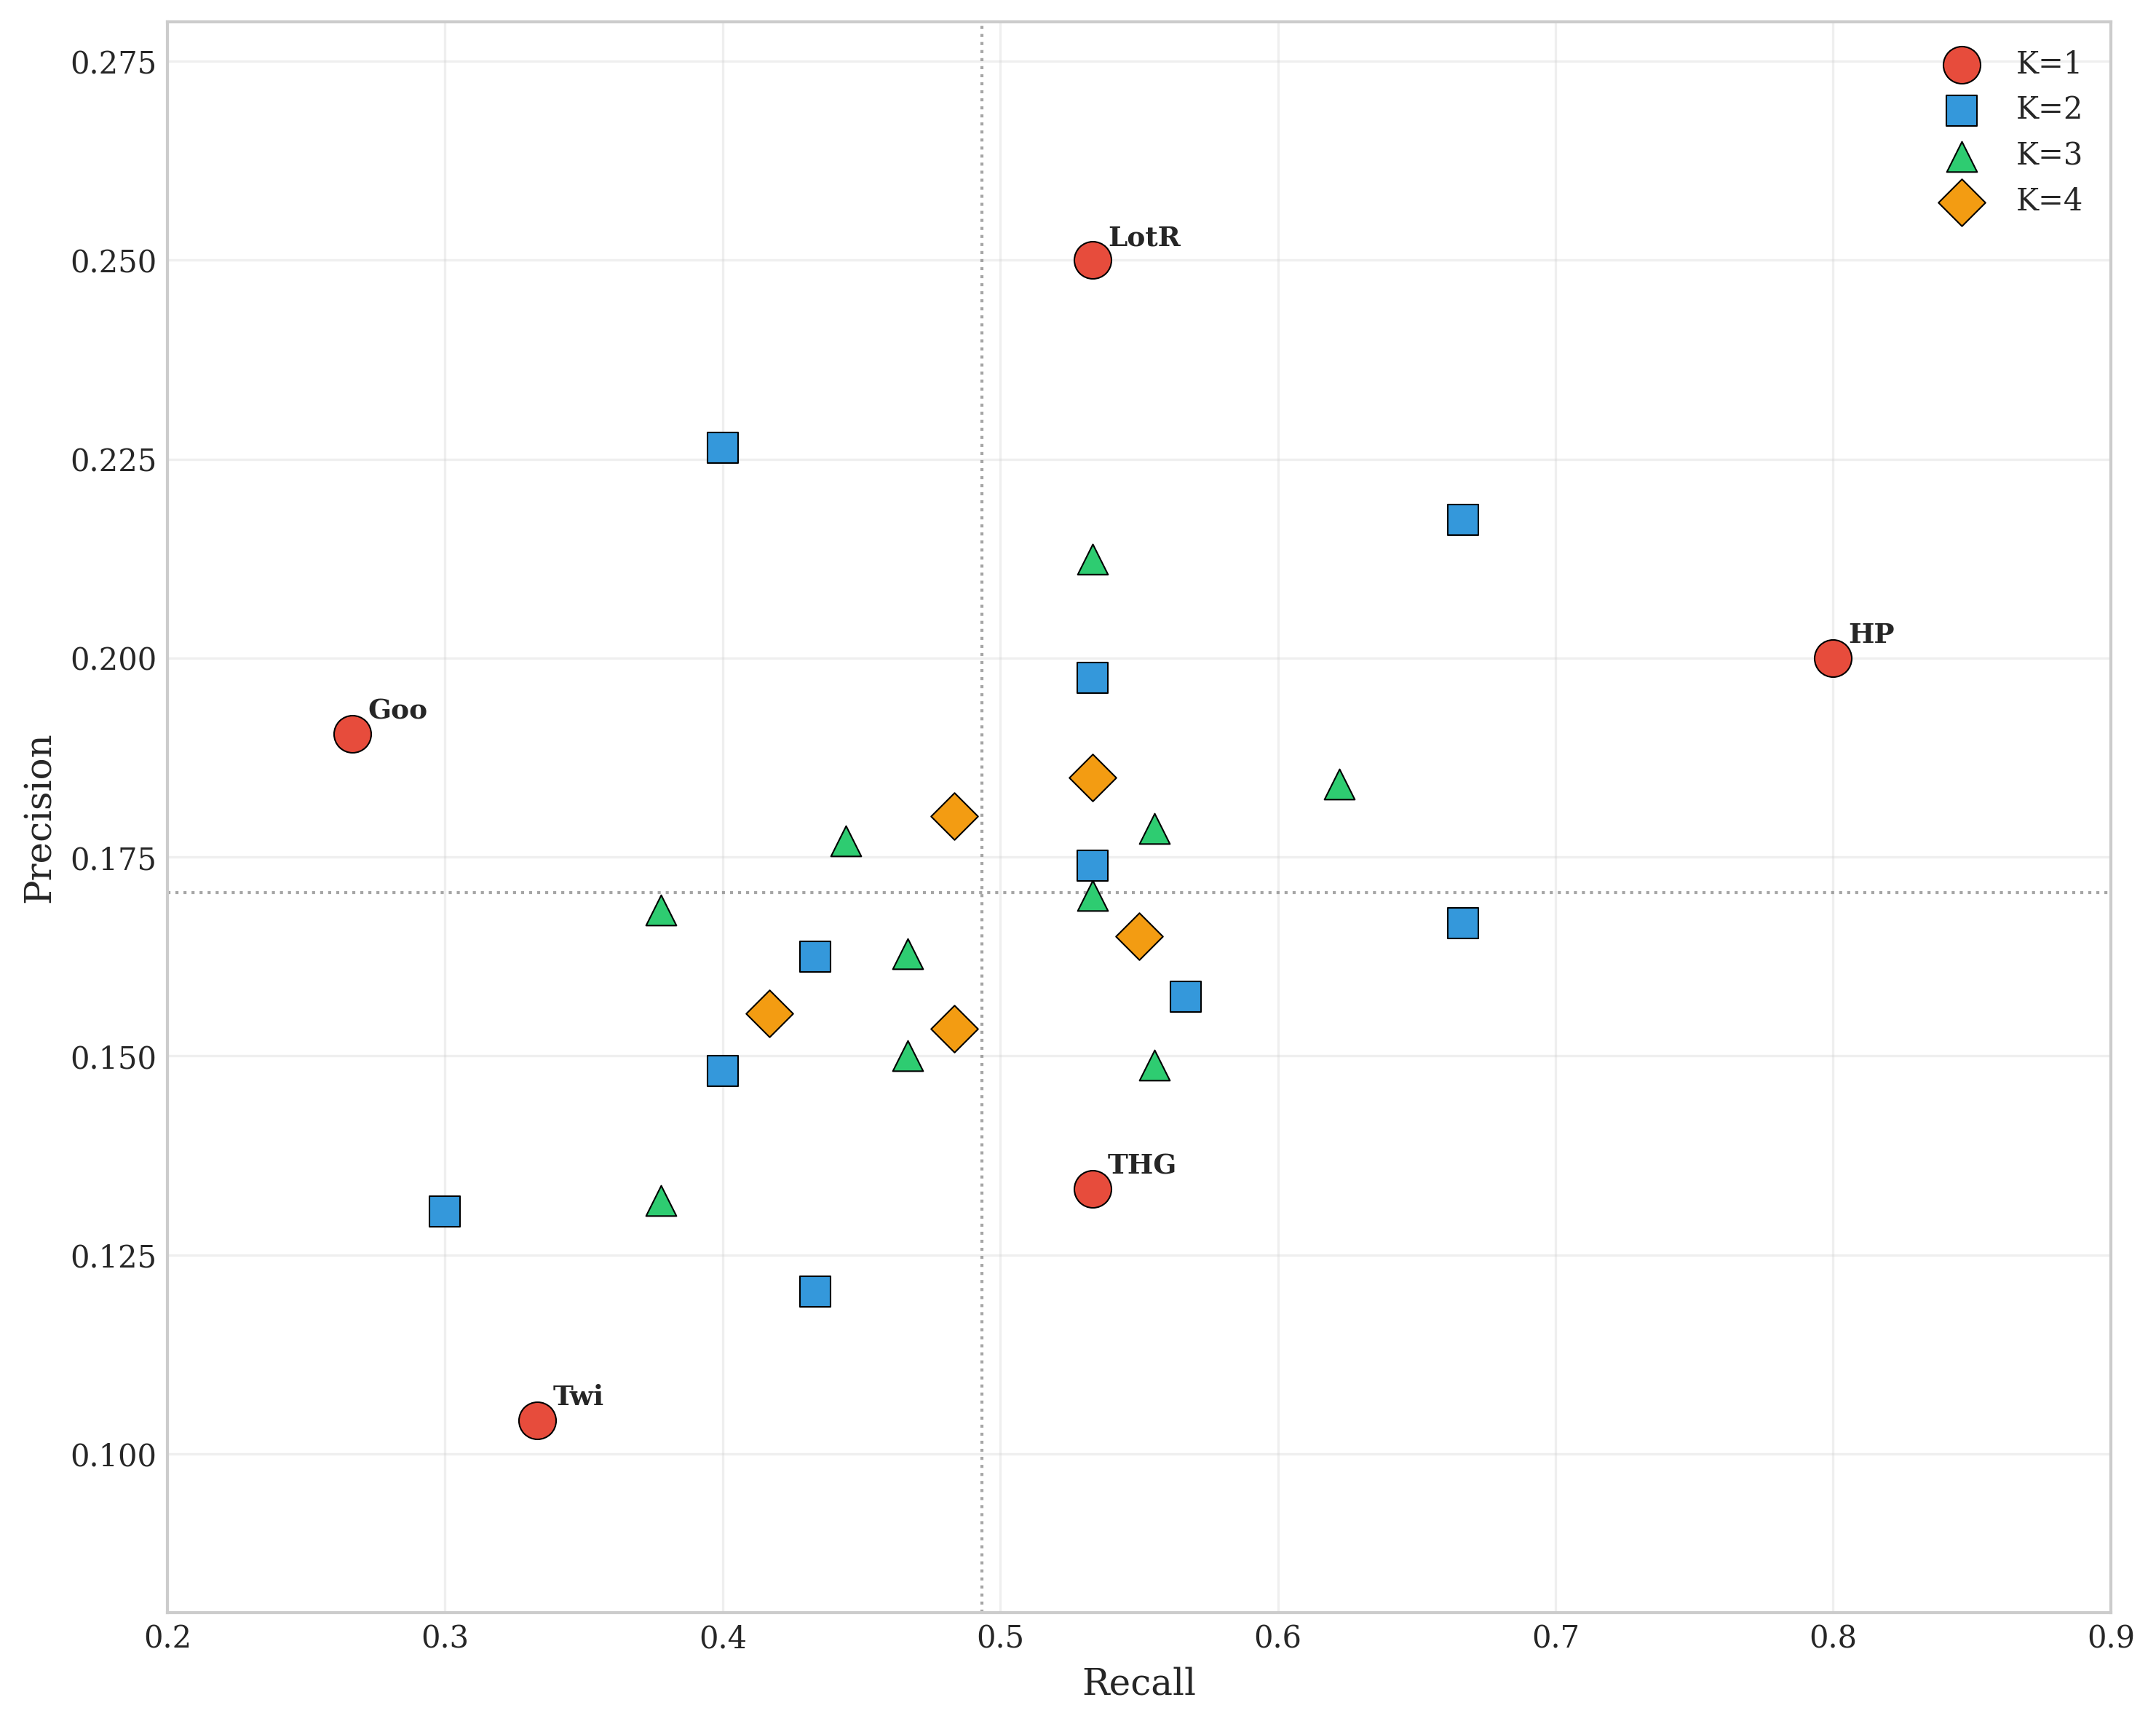
\includegraphics[width=0.95\textwidth]{figures/plot6_precision_recall_scatter.png}
\caption{Precision-recall trade-off across all 30 experiments. Each point represents one experiment configuration, with marker shape indicating the k value. Points cluster around (0.45--0.55 recall, 0.15--0.22 precision), with outliers at high recall/low precision (Harry Potter at k=1, labeled ``HP'') and lower recall/higher precision (Goosebumps and Lord of the Rings combinations). The dotted gray lines indicate overall average recall (49.33\%) and precision (17.05\%). The clustering confirms that detection performance is bounded by fundamental limitations in the extraction data rather than random variation.}
\label{fig:precision_recall_scatter}
\end{figure}

Figure~\ref{fig:precision_recall_scatter} plots the precision-recall trade-off for all 30 experiments. Points cluster around (0.45-0.55 recall, 0.15-0.22 precision), with outliers at high recall/low precision (Harry Potter at k=1) and lower recall/higher precision (Goosebumps+LotR combinations). The clustering confirms that detection performance is bounded by fundamental limitations in the extraction data rather than random variation.

\begin{figure}[htbp]
\centering
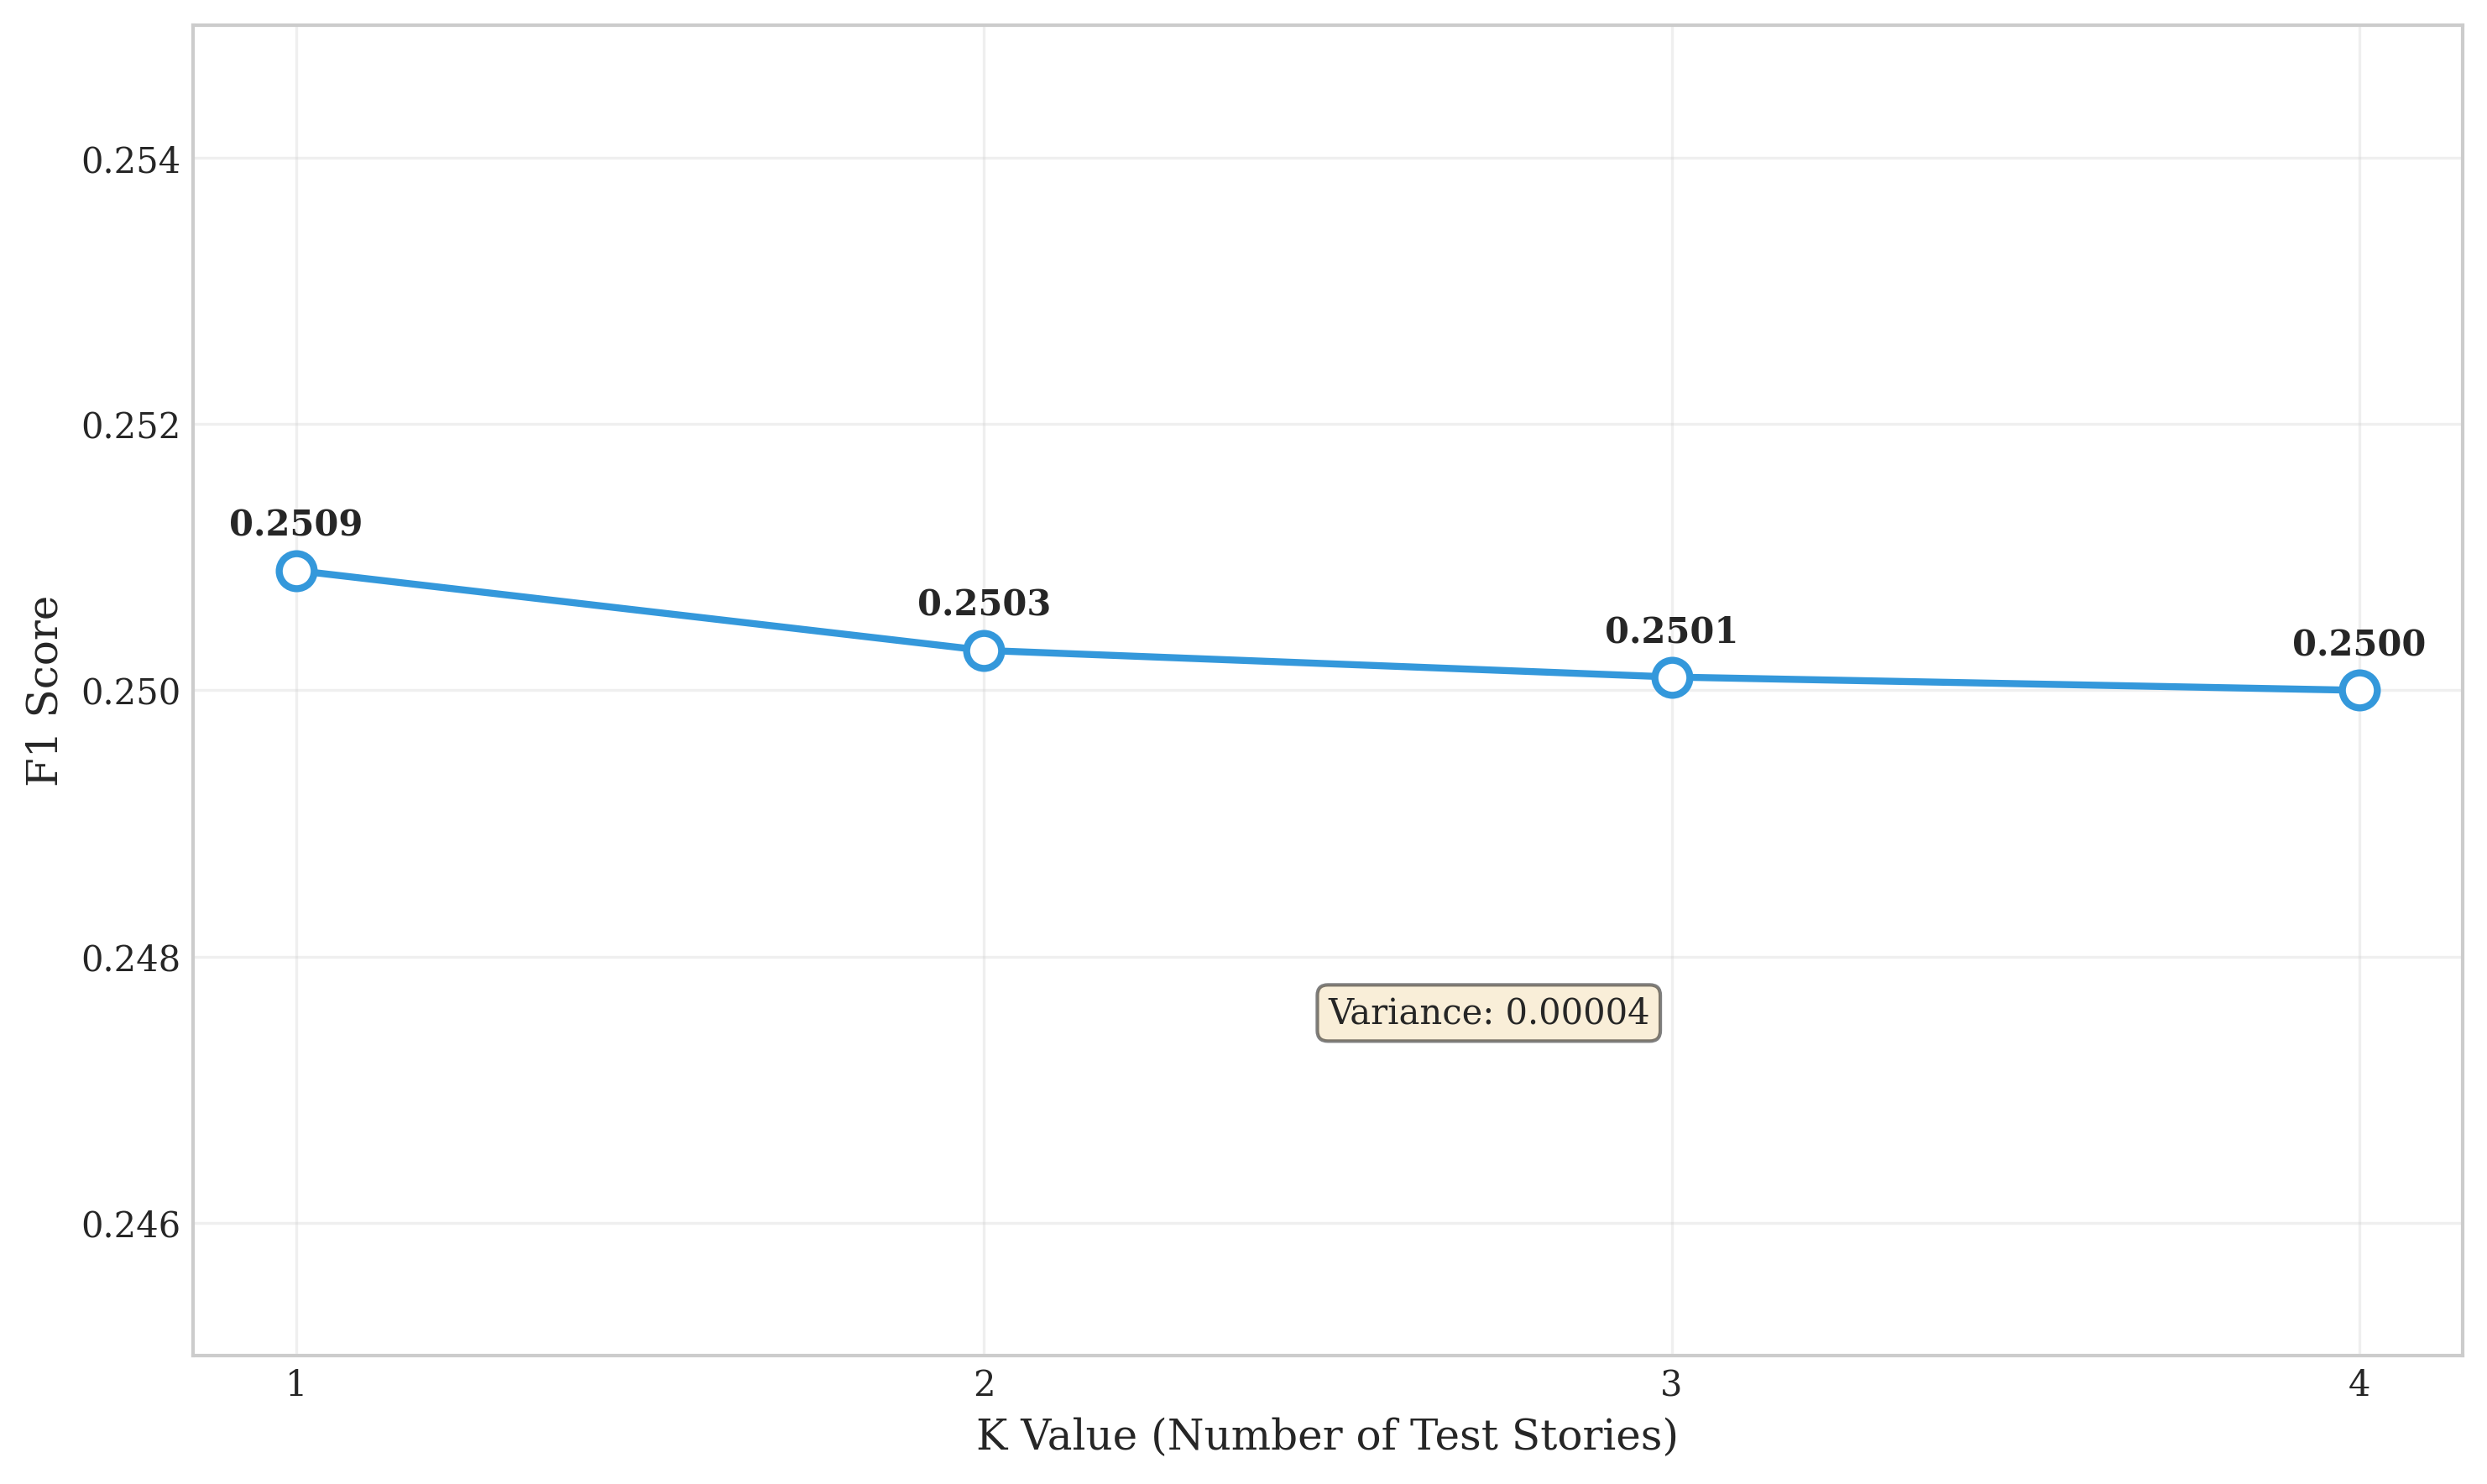
\includegraphics[width=0.95\textwidth]{figures/plot8_f1_stability.png}
\caption{F1 score stability across k-fold configurations. The F1 score varies by only 0.0009 across all four k values (from 0.2509 at k=1 to 0.2500 at k=4), demonstrating exceptional stability and indicating that the detection rules generalize uniformly across different story combinations rather than overfitting to specific narratives. This stability suggests that performance is determined by fundamental rule characteristics rather than training set composition.}
\label{fig:f1_stability}
\end{figure}

Figure~\ref{fig:f1_stability} demonstrates the remarkable stability of F1 scores across k values, varying by only 0.0009 (from 0.2509 at k=1 to 0.2500 at k=4). This stability indicates that the detection rules generalize uniformly across story combinations, confirming that performance is determined by fundamental rule characteristics rather than overfitting to specific training configurations.

\begin{figure}[htbp]
\centering
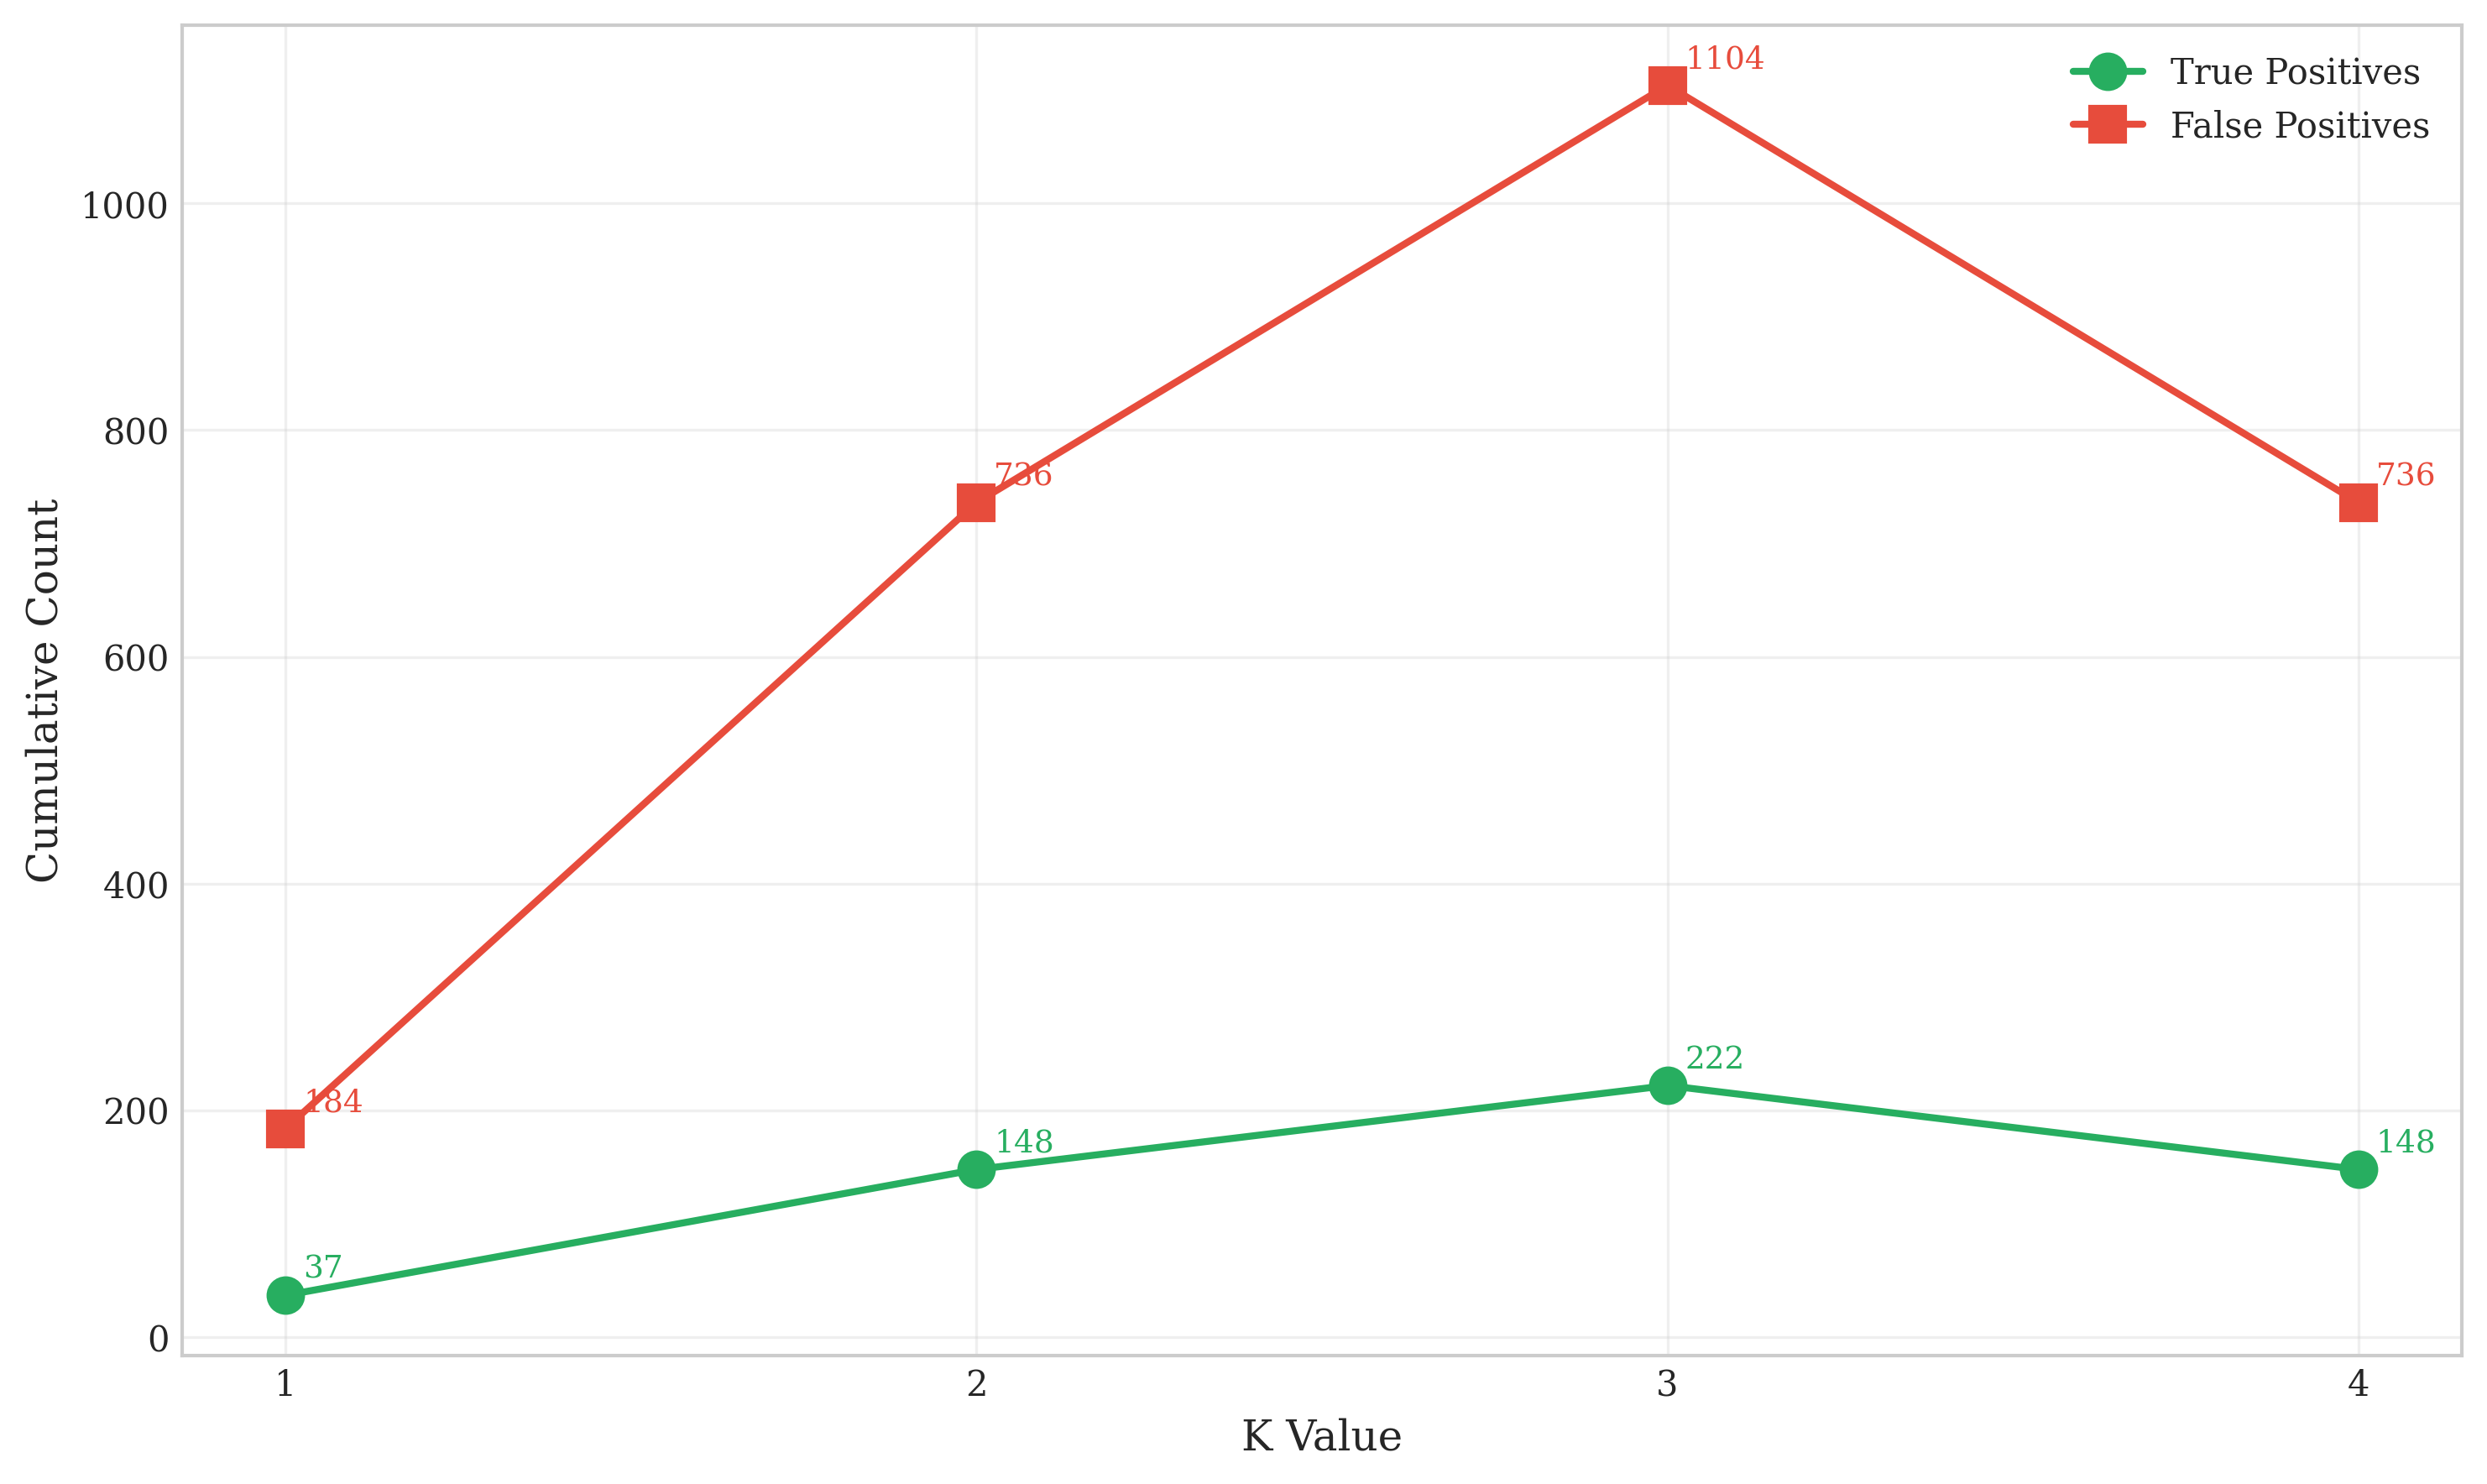
\includegraphics[width=0.95\textwidth]{figures/plot10_cumulative_tp_fp.png}
\caption{Cumulative true positives and false positives across k values. The pattern reflects the number of test stories evaluated in each configuration: k=3 evaluates the most stories across its 10 experiments (450 total GT), while k=1 and k=4 each evaluate 75 GT errors per configuration but with different numbers of experiments (5 each). The ratio of FP to TP remains approximately constant at 5:1, confirming that precision does not improve with larger evaluation sets.}
\label{fig:cumulative_tp_fp}
\end{figure}

Figure~\ref{fig:cumulative_tp_fp} shows cumulative true positives and false positives across k values. The FP to TP ratio remains approximately constant at 5:1 regardless of k value, confirming that precision does not improve with larger evaluation sets. This stability indicates that the precision limitation is fundamental to the detection approach rather than an artifact of small sample sizes.

The qualitative analysis of detection successes and failures reveals systematic patterns. Successful detections predominantly fall into three categories: (1) appearance anomalies where modified text introduces unusual colors or states (e.g., ``pale green'' face, ``grayish white'' complexion), which the abnormal\_appearance rules directly detect; (2) relationship-action contradictions where hostile characters perform warm actions or friendly characters perform hostile actions, triggering the relationship\_action\_mismatch rules; and (3) chapters with high concentrations of unusual social interactions that exceed the multi-signal threshold.

Detection failures cluster around errors requiring reasoning capabilities absent from the current system. Temporal Order errors (26.67\% recall) typically involve sequence violations that require tracking event order across paragraphs or chapters. For example, Harry Potter Chapter 27 contains an error where ``Harry already got into the stall'' contradicts the subsequent text ``unlocked the stall again to get in''---detecting this requires understanding that entering a stall must precede being inside it. Location Correctness errors (46.67\% recall) frequently involve spatial impossibilities (``cannot reach dormitory from dungeon'') that require a map-like understanding of story geography not present in the extraction. Basic Coherence errors with moderate recall (46.67\%) include physical impossibilities that vary in detectability: color anomalies are caught, but errors like ``bowl cannot be both full and spilled'' require semantic understanding of object states.

The multi-signal detection approach represents an attempt to capture errors through co-occurrence of suspicious patterns rather than direct rule matching. While this increases recall (contributing 27 of 37 true positives), it fundamentally cannot distinguish between chapters with legitimate narrative complexity and chapters with coherence errors, as the extracted signals (hostile relationships, negative emotions, social conflicts) appear in roughly similar proportions in both ground truth and non-ground truth chapters. The differential of only 8\% for the most discriminative signal (hostile\_pair presence) explains why precision remains low regardless of threshold tuning.

The experimental results establish clear upper bounds on detection performance achievable with the current extraction pipeline. The 49.33\% recall ceiling reflects that approximately half of injected errors manifest in ways that produce detectable signals in the extraction data. The 17.56\% precision floor reflects that the same signals appear frequently in non-error chapters due to normal narrative complexity. Achieving the target metrics of 80\% recall and 60\% precision would require fundamental enhancements to the extraction pipeline, including spatial relationship modeling, temporal sequence tracking, and deeper semantic understanding of physical and logical constraints.

\begin{table}[htbp]
\centering
\caption{Summary of Key Findings. This table consolidates the primary experimental results and their supporting evidence.}
\label{tab:summary_findings}
\begin{tabular}{lp{10cm}}
\toprule
\textbf{Finding} & \textbf{Evidence} \\
\midrule
Stable generalization & Recall constant at 49.33\% across all k values (variance $<$ 0.0001) \\
Story-dependent performance & Recall ranges from 26.67\% (Goosebumps) to 80.00\% (Harry Potter) \\
Category-dependent detection & Temporal Order worst (26.67\%), Causality/Emotional best (60.00\%) \\
Precision-recall trade-off & Higher recall configurations incur proportionally higher FP rates \\
Signal weak discriminability & Best discriminating signal shows only 8.07\% differential \\
Rule specialization & abnormal\_appearance achieves 41.67\% precision; multi\_signal achieves 23.28\% \\
Upper bound on performance & Current extraction limits recall to $\sim$50\%, precision to $\sim$18\% \\
\bottomrule
\end{tabular}
\end{table}

Table~\ref{tab:summary_findings} summarizes the key findings from our experimental evaluation. The logic-based narrative coherence detection system demonstrates stable generalization across story combinations but reveals fundamental limitations in achievable performance metrics. The results indicate that substantial improvements would require not rule refinement but extraction pipeline enhancement to capture the spatial, temporal, and semantic information necessary for detecting the majority of coherence error types.
